\documentclass[a4paper,11pt]{book}

%%%%%%%%%%%%%%%%%%%%%%%%%%%%%%%%%Les packages%%%%%%%%%%%%%%%%%%%%%%%%%%%%%%%%%%%%%%
\usepackage[utf8]{inputenc}%           gestion des accents (source)
\usepackage[T1]{fontenc}%              gestion des accents (PDF)
\usepackage[english,french]{babel}
%\usepackage[francais]{babel}%          gestion du français
\usepackage{textcomp}%                 caractères additionnels
\usepackage{listings}%                 pour insérer du code source
\usepackage{amssymb,amsthm,amsmath,amsfonts,mathrsfs}% packages de l'AMS + mathtools
\usepackage{lmodern}%                  police de caractère
\usepackage{geometry}%                 gestion des marges
	\geometry{papersize={21cm,29.7cm}}
	\geometry{margin=2cm,bottom=2cm}
\usepackage{graphicx}%                 gestion des images
	\graphicspath{{images/}}%pour spécifier le chemin d'accès aux images
\usepackage{xcolor}%                   gestion des couleurs
\usepackage{array}%                    gestion améliorée des tableaux
\usepackage{tgpagella}%
\usepackage{calc}%                     syntaxe naturelle pour les calculs
\usepackage{titlesec}%                 pour les sections
\usepackage{titletoc}%                 pour la table des matières
\usepackage{fancyhdr}%                 pour les en-têtes
\usepackage{titling}%                  pour le titre
\usepackage{enumitem}%                 pour les listes numérotées
\usepackage[breaklinks]{hyperref}%                 gestion des hyperliens, rend actif les liens, références croisées,
\hypersetup{pdfstartview=XYZ}%         zoom par défaut
%\usepackage{abstract}%
\usepackage{stmaryrd}% 				   pour délimiteurs ouvrants et fermants
\usepackage{footmisc}%
\usepackage{multirow}%				   Fusion de cellules
\usepackage{pdfpages}%					Pour inclure des pages entières d’un PDF
\usepackage{caption}%					placement manuel d'image
%\usepackage{mathdots}%permet d’avoir des points de suspension corrects en indice ou exposant.
\usepackage{shorttoc}%                  pour la réalisation d'un sommaire
\usepackage{remreset}%
\usepackage{pgf,tikz}%             gestion des dessins  
	\usetikzlibrary{arrows}
\usepackage{eurosym}%
\usepackage{soul}%
\usepackage{bookman}
\usepackage{ wrapfig}
\usepackage{ulem}
\usepackage{ setspace}
\usepackage{ layout}
\usepackage{lipsum}% juste utile ici pour générer du faux texte}
%\usepackage{mwe}%juste utile ici pour générer de fausses images
\usepackage[Rejne]{fncychap}%pour de jolis titres de chapitres voir la doc pour d'autres styles.
\usepackage{soul}
\usepackage{float}
%%%%%%%%%%%%%%%%%%%style main%%%%%%%%%%%%%%%%%%%%%%%%%%%%%%%%%%%%
        \fancypagestyle{mainmatter} {}
                \fancyhf{}
                \fancyhead[R]{\leftmark} % Right Even
                \fancyfoot[C]{\thepage}
                %\fancyfoot[C]{\thepage \\\scriptsize Conception et développement d’une plateforme communautaire de découverte d’expérience et de location à court terme d’appartement ou de parties d’appartement entre particuliers}
               
             
\renewcommand{\headrulewidth}{1.5pt}%trait horizontal pour l'en-tête
        \renewcommand{\footrulewidth}{2pt}%trait horizontal pour les pieds de pages              
%%%%%%%%%%%%%%%%%%%%%%%%%%%%%%%%%%%%%%%%%%%%%%%%%%%%%%%%%%%%%%%%%%%%%%%%%%%%%%%%%%%%%%%%%%%%%%%%%%%%%%%%%%%%%%%%%%%%%%%%%%%%%%%%%%%%%%%%%%%%
  \setlength{\headheight}{14.2pt}% hauteur de l'en-tête
\usepackage{ makeidx} 
\usepackage[french]{nomencl}
\lstnewenvironment{ccode}[1][]
  {\lstset{language=C,numbers=left,numberstyle=\tiny,#1}}
  {}
\lstset{aboveskip=\topsep,belowskip=\topsep,
        frame=single,rulecolor=\color{black}}%,backgroundcolor=\color{blue!5}}
        
%%%%%%%%%%%%%%%%%%%style back%%%%%%%%%%%%%%%%%%%%%%%%%%%%%%%%%%%%%%%%%  
        \fancypagestyle{backmatter}{%
                \fancyhf{}%on vide les en-têtes
                \fancyfoot[C]{ \thepage}%
                \renewcommand{\headrulewidth}{1.5pt}%trait horizontal pour l'en-tête
                \renewcommand{\footrulewidth}{2pt}%trait horizontal pour les pieds de pages
                }
                
 %%%%%%%%%%%%%%%%%%%%%%%%%%%%%%%%%%%%%%%%%%%%%%%%%%%%%%%%%%%%%%%%%%
\makenomenclature
\renewcommand{\nomname}{Liste des abréviations, des sigles et des symboles}
\makeatletter
\newenvironment{abstract}{%
    \cleardoublepage
    \null\vfil
    \@beginparpenalty\@lowpenalty
    \begin{center}%
      \bfseries \abstractname
      \@endparpenalty\@M
    \end{center}}%
   {\par\vfil\null}
\makeatother
 %%%%%%%%%%%%%%%%%%%style front%%%%%%%%%%%%%%%%%%%%%%%%%%%%%%%%%%%%%%%%% 
        \fancypagestyle{frontmatter}{
                \fancyhf{}%on vide les en-têtes
                \fancyfoot[C]{ \thepage}%
                \renewcommand{\headrulewidth}{1.5pt}%trait horizontal pour l'en-tête
                \renewcommand{\footrulewidth}{2pt}%trait horizontal pour les pieds de pages
                }
%%%%%%%%%%%%%%%%%%%%%%%%%%%%index%%%%%%%%%%%%%%%%%%%%%%%%%%%%%%%%%%%%%%%
\makeindex
                \hypersetup{colorlinks,%
                citecolor=black,%
                filecolor=black,%
                linkcolor=black,%
                urlcolor=black} 
%%%%%%%%%%%%%%%%%%%%%%%%%%%%%% les environnements %%%%%%%%%%%%%%%%%%%%%%%%%%%%%%%%%%%%%%%
\newcounter{exos}[section]
 \newenvironment{exos}{\stepcounter{exos}\vspace{0.5cm}{\center{\bfseries\ul{Exercice  \theexos}}}}{\par\vspace{0.5cm}}
\newcounter{sol}[section]
 \newenvironment{sol}{\stepcounter{sol}\vspace{0.5cm}{\center{\bfseries \ul{Solution  \thesol}}}}{\par\vspace{0.5cm}} 


%%%%%%%%%%%%%%%%%%%%%%%%%%%%%%%%%%%%%%%%  setting  page and marges %%%%%%%%%%%%%%%%%%%%%%%%%

 %\linespread{1.2}%{1.4}% this is for the intervall between lines
%%%%%%%%%%%%%%%%%%%%%%%%%%%%biblio%%%%%%%%%%%%%%%%%%%%%%%%%%%%%%%%%%%%
%\usepackage[backend=biber]{biblatex}
%\addbibresource{bibliographie/biblio.bib}% pour indiquer où se trouve notre .bib
\usepackage{csquotes}% pour la gestion des guillemets français.
\usepackage{nomencl}
\makenomenclature
\renewcommand{\nomname}{Liste des abréviations, des sigles et des symboles}

%%%%%%%%%%%%%%%%%%%%%%%%%%%%%%%%%%%%%%%%%%%%%%%%%%%%%%%%%%%%%%%%%%%
\usepackage{draftwatermark}
	\SetWatermarkLightness{0.8}
	\SetWatermarkAngle{25}
	\SetWatermarkScale{2}
	\SetWatermarkFontSize{1cm}
	\SetWatermarkText{} 
	
%%%%%%%%%%%%%%%%%%%%%%%%%%%%%%%%%%%%%%%%%%%%%%%% chapter style defined %%%%%%%%%%%%%%%%%%%%%%%%%%%%%%%%%%%
\titleclass{\subsubsubsection}{straight}[\subsection]

\newcounter{subsubsubsection}[subsubsection]
\renewcommand\thesubsubsubsection{\thesubsubsection.\arabic{subsubsubsection}}

\titleformat{\subsubsubsection}
  {\normalfont\normalsize\bfseries}{\thesubsubsubsection}{1em}{}
\titlespacing*{\subsubsubsection}
{0pt}{3.25ex plus 1ex minus .2ex}{1.5ex plus .2ex}

\makeatletter

\def\toclevel@subsubsubsection{4}
\def\l@subsubsubsection{\@dottedtocline{4}{7em}{4em}}
\makeatother

\setcounter{secnumdepth}{4}
\setcounter{tocdepth}{4}
                              
%%%%%%%%%%%%%%%%%%%%%%%%%%%%%%%%%%%%%%%%%%%%%%%%%%%%%%%%%%%%%%%%%%%%%%%%%%

\begin{document}

\pagestyle{fancy} %style des en-têtes pour cette partie
\let\cleardoublepage\clearpage

\frontmatter % d\'ebut des pages liminaires

\begin{titlepage}


\includegraphics[width=3.5cm]{images/benin.png}\qquad\qquad\qquad
\textsc{\textbf{République du Bénin}}\qquad\qquad\quad 
\includegraphics[width=4cm]{images/esgis.jpg}

\begin{center}
\textsc{\textbf{Ministère de l'Enseignement Supérieur et de la Recherche Scientifique}}
\\$ $\\ \textsc{\textbf{Direction Générale de l'Enseignement Supérieur Privé}}
\end{center}

\vspace*{1cm}

\begin{center}
\bf{\large{\'Ecole Supérieur de Gestion d’Informatique et des Sciences (ESGIS - Bénin)}}
\end{center}

\parindent=0pt
\definecolor{bordeaux}{rgb}{.5,0,0}\small {} 

\vspace*{\stretch{1}}
\hspace{4cm}


\begin{center}
\textsc{\large{\textbf{Mémoire de fin de formation}}} 
\end{center}

\begin{center} Pour l'obtention du Diplôme de Licence en Informatique\end{center}

\begin{center}Option: \bf{Architecture logicielle}
\end{center}

\vspace*{1cm}

\vspace*{\stretch{1}}
\rule{17cm}{3pt}
\begin{center}\bfseries\Large
   \textit{Conception et développement d’une plateforme  de location court durée d’appartements entre particuliers} 
\end{center}
\rule{17cm}{3pt}

    
\[\]

\begin{center}
Réalisé par : 
\end{center}

\begin{center}
\textbf{Kenneth ASSOGBA}
\end{center}

\[\]

Maître de mémoire: \qquad\qquad\qquad\qquad\qquad\qquad\qquad\qquad\qquad\qquad\qquad\qquad\qquad\qquad \quad Maître de stage:
\\\\\bf{M. Juste AHOUANDJINOU} \qquad\qquad\qquad\qquad\qquad\qquad\qquad\qquad\qquad\qquad\qquad\qquad   \quad\bf{ M. Hakim OUAK\'E}
 
    \vspace*{3cm}

     \begin{center}
     \textbf{Ann\'ee Universitaire:} 2016-2017
     \end{center}
     \vspace*{3cm}

 \end{titlepage}%on cr\'ee la couverture
\thispagestyle{empty}%pour la page de garde toute blanche

\chapter{Dédicaces}
\textit{Je dédie ce mémoire
\\$ $\\À ma très chère famille, principalement mes parents. Aucune dédicace ne
saurait être assez éloquente pour exprimer ce que vous méritez pour tous
les sacrifices que vous n’avez cessé de consentir pour moi depuis ma
naissance jusqu’aujourd’hui.
\\Puisse Dieu, le tout puissant, vous préserver et vous accorder santé ,
longue vie et bonheur.
\\$ $\\À mon frère défunt. La mort n’arrête pas l’amour.}%no comment !
\chapter{Remerciements}
\textit{J’exprime ma profonde gratitude à :}
\begin{itemize}
\item[•]\textit{Mon maître de mémoire, Mr. Juste AHOUANDJINOU , qui m’a témoigné d’une grande considération et d’une disponibilité inattendue malgré ses multiples occupations};
\item[•]\textit{Mon maître de stage Mr. Hakim OUAKÉ , pour son encadrement et la disponibilité dont il a fait preuve durant tout mon stage};
\item[•]\textit{Mr. Boris DEHOUMON, pour m’avoir inspiré ce thème et suivi la réalisation du projet};
\item[•]\textit{Tout le personnel de EtriLabs Cotonou pour avoir su partager son savoir faire et pour avoir mis à ma disposition les outils nécessaires au bon déroulement de ce stage};
\item[•]\textit{Toute l’administration de l'Ecole Supérieure de Gestion d'Informatique et des Sciences (ESGIS) pour leur contribution à ma formation};
\item[•]\textit{Tous mes camarades de promotion et en particuliers ceux avec qui j’ai eu à travailler pour leur aide et leurs différentes suggestions apportées au cours du développement de notre projet}
\end{itemize}
 %no comment !

\renewcommand{\contentsname}{Table des matières}
\cleardoublepage
\phantomsection
\addcontentsline{toc}{chapter}{Sommaire}%ajout du sommaire dans le sommaire !
\shorttoc{Sommaire}{1}
\thispagestyle{frontmatter}

\chapter{Liste des sigles et abréviations}
\begin{itemize}
\item[\textbullet] API : Application programming Interface
\item[\textbullet] CSS : Cascading Style Sheet
\item[\textbullet] DaaS : Database as a Service
\item[\textbullet] EtriLabs: Educational Technology and Research International Laboratory
\item[\textbullet] HTML : HyperText Markup Language
\item[\textbullet] HTTP : HyperText Transfert Protocol
\item[\textbullet] JSON : JavaScript Object Notation
\item[\textbullet] NoSQL : Not Only SQL
\item[\textbullet] NPM : Node Package Manager
\item[\textbullet] PaaS : Platform as a Service
\item[\textbullet] REST : Representationnal State Transfert
\item[\textbullet] SGBD : Système de Gestion de Base de Données
\item[\textbullet] SQL : Structured Query Language
\item[\textbullet] UI : User Interface
\item[\textbullet] UML : Unified Modeling Language
\item[\textbullet] WHISPA : Women High Impact Startup Preparation Academy
\end{itemize}

\cleardoublepage
\phantomsection
\addcontentsline{toc}{chapter}{Liste des tableaux}
\listoftables

\cleardoublepage
\phantomsection
\addcontentsline{toc}{chapter}{Table des figures}
\listoffigures

\chapter{Résumé/Abstract}
\begin{flushleft}\textbf{Résumé}\end{flushleft}
Lorsque nous voyageons à l'intérieur du territoire béninois, un choix presque binaire se présente à nous pour le logement: loger chez un proche ou dans un hôtel. Cette faible offre pénalise de nombreux voyageurs. Loger chez un proche n'est pas toujours simple, loger dans un hôtel est cher et peu convivial. D'autre part, de nombreux particuliers disposent de logements inoccupés et souhaiteraient pouvoir en tirer un gain régulier tout en ayant aussi la possibilité d’en disposer au moment voulu. Par ailleurs, sans que cela ne constitue toutefois le but premier de son voyage, tout voyageur désire faire de son séjour une expérience unique. Il choisit donc sa destination selon les différentes attractions culturelles ou les expériences particulières qu’elle offre. Ce mémoire de fin de formation se propose d’offrir un outil en ligne permettant de mettre en contact direct deux particuliers: un hôte local et un voyageur à la quête d'un logement convivial à prix raisonnable ou d'une expérience unique. Ainsi, la mise en place d’une plateforme communautaire de découverte d'expérience thématique et de location à court terme d’appartements ou de parties d’appartements entre particuliers, implémentée avec la pile logicielle JavaScript moderne: NodeJs, NPM, React, Webpack, Babel, Ionic sera profitable  pour satisfaire les attentes des diverses clientèles. Cela permettra en effet d'une part aux voyageurs de réserver un logement ou de s’inscrire à une expérience thématique ; d'autre part aux hôtes de mettre en location un appartement ou de proposer une expérience. 
\\$ $\\ \textbf{Mots Clés}: location courte durée, expérience thématique, voyage, tourisme, culture
\newpage
$ $\\$ $\\$ $\\$ $\\$ $\\$ $\\$ $\\$ $\\$ $\\$ $\\$ $\\$ $
\textbf{Abstract}
\\When we travel within the Beninese territory, an binary choice comes to us for housing: staying with family or in a hotel. This low offer penalizes many travelers. Staying with family is not always easy, staying in a hotel is expensive and not very friendly. On the other hand, many individuals have vacant dwellings and wish they could make a steady gain while also having the opportunity to dispose of them at the right time. Moreover, without this being the primary purpose of his trip, any traveler wishes to make his stay a unique experience. He therefore chooses his destination according to the different cultural attractions or the particular experiences that it offers. This end-of-study dissertation proposes to offer an online tool to put two private individuals in direct contact: a local host and a traveler in search of a reasonably priced, comfortable accommodation or a unique experience. Thus, the establishment of a community platform for discovery of thematic experience and short-term rental of apartments or portions of apartments between individuals, implemented with the modern JavaScript software stack: NodeJs, NPM, React, Webpack , Babel, Ionic will be profitable to meet the expectations of various customers. This will allow travelers to book accommodation or register for a thematic experience; On the other hand, guests can rent an apartment or offer an experience.
\\$ $\\ \textbf{Key words}: short-term rental, thematic experience, travel, tourism, culture
\thispagestyle{frontmatter}

\mainmatter% corps du document

\cleardoublepage
\phantomsection
 \addcontentsline{toc}{chapter}{Introduction}
\chapter*{Introduction}
Les ordinateurs et terminaux mobiles ont connu durant les dernières années une évolution exponentielle en termes de performance et de fonctionnalités. Cela a préparé le terrain pour des usages assez avancés de la technologie, spécifiquement dans le développement d’applications web et mobile, capables de répondre aux attentes de plus en plus grandissantes du public.

Les béninois utilisent de plus en plus les systèmes numériques, confirmant ainsi la véritable révolution technologique que vivent depuis quelques années, tous les secteurs d’activité de notre pays. Les secteurs de la culture et du tourisme en particulier sont en plein essor et présentent un avantage particulier pour l’innovation. 

Malgré ses avancées, il semble difficile d’apporter un regard neuf sur la richesse touristique béninoise. De plus, le logement au Bénin reste une difficulté, même pour les nationaux en déplacement à l'intérieur du territoire. Face à cette situation, il est important de trouver une solution adéquate permettant de répondre au mieux aux besoins du secteur du logement et du tourisme au Bénin.

C’est dans ce contexte que s’inscrit le présent projet intitulé : “Conception et développement d’une plateforme  de location court durée d’appartements entre particuliers”. Il comprend quatre (04) chapitres. Le premier chapitre est consacré à la description du cadre de notre stage, le deuxième au contexte de l’étude et à l’état de l’art. Le troisième chapitre intitulé « Analyse, Conception et Choix Techniques » présente une proposition de solution, le choix de la méthode d'analyse, l’analyse fonctionnelle et conceptuelle ainsi que le choix des outils d'implémentation et l’architecture du système. Le quatrième et dernier chapitre intitulé « Réalisation de l’application », décrit les interfaces développées côté client, le serveur et la base de données de l’application.

\chapter{Description institutionnelle d’EtriLabs}
Notre stage s’est déroulé à l’ONG EtriLabs Cotonou. Cette partie aborde l’historique de notre structure d’accueil, le rôle et les différentes activités que nous y avons effectuées ainsi que les compétences que nous avons acquises dès lors.

\section{Présentation de l'entreprise}

\subsection{Historique de l’entreprise}
Educational Technology and Research International (ETRI) opérant sous le nom commercial EtriLabs, est une Organisation Non-Gouvernementale qui se sert des Technologies de l’Information et de la Communication (TIC) pour intervenir dans plusieurs domaines. Elle a été créée en 2010 pour pallier entre autres, le retard de l’Afrique et du Bénin en particulier dans le domaine du numérique. Son objectif étant de promouvoir la culture de l’innovation et de la compétitivité en incluant toutes les couches sociales, elle a pour mission de faire la promotion des TIC au service du développement.

\subsection{Organisation de l’entreprise}
EtriLabs est présente dans deux pays d’Afrique : le Bénin et le Sénégal. Au Bénin elle est présente à Parakou et à Cotonou où se trouve son siège officiel. De façon générale, quatre niveaux hiérarchiques s’y succèdent. Nous avons donc:

\paragraph{Le Président Directeur Général}
$ $\\Le Président Directeur Général de EtriLabs est le représentant légal de l’entreprise. Il préside le conseil d’administration. En cette qualité:
\begin{itemize}
\item[\textbullet] Il définit ses objectifs généraux et décide en dernier ressort des moyens financiers, matériels et humains à mettre en œuvre dans le cadre des orientations et des décisions du conseil d’administration ;
\item[\textbullet] Il anime le comité de direction de l’entreprise et est responsable de ses résultats ;
\item[\textbullet] Il est chargé de la gestion des contrats avec les partenaires ;
\item[\textbullet] Il est enfin chargé de la culture de l’organisation.
\end{itemize}

\paragraph{Le Directeur Technique}
$ $\\Le directeur technique supervise l'ensemble des projets de l’entreprise, depuis l'étape de la conception jusqu'au support. Il est concrètement chargé de :
\begin{itemize}
\item[\textbullet] mesurer les retours sur investissement ;
\item[\textbullet] définir ou de réorienter une nouvelle stratégie d'entreprise en fonction des résultats ;
\item[\textbullet] établir des programmes de recherche et de développement puis d’apporter des idées quant aux nouveaux produits et procédés ;
\item[\textbullet] coordonner le développement des produits en concordance avec la réglementation en matière de qualité de sécurité et d'environnement.
\end{itemize}

\paragraph{Le Directeur des Programmes}
$ $\\Le Directeur des Programmes de EtriLabs, supervise la coordination et l'administration de tous les aspects des programmes de EtriLabs, y compris la planification, l'organisation, la dotation, la conduite et le contrôle des activités des programmes.
Il gère l'implantation financière, logistique et journalière des programmes WHISPA, TEKLIONS et Learn2Code.

\paragraph{L’Agent des Programmes} 
$ $\\L’Agent des Programmes de EtriLabs Cotonou est chargée de :
\begin{itemize}
\item[\textbullet] Construire et développer des relations avec les partenaires stratégiques et la communauté ;
\item[\textbullet] Gérer, planifier, coordonner et superviser les activités, les événements, les séances de formation et les programmes;
\item[\textbullet] Contribuer à la conception et au développement de propositions de projets.
\end{itemize}

EtriLabs Cotonou offre plusieurs services dont l’incubation et l’accélération de startups. Les équipiers de ces startups représentent en majorité son personnel. Au nombre de ces startups nous avons : Pikiz, Intside, Queezly, Chaperone, ClassAction, HappierCo, Sewema, BeninMaison, Mentorat Club, Socializer et Botamp.
\\Ces dernières ont chacune une structure propre. La taille des équipes varie de deux à six équipiers desquels on dénombre des développeurs et d’autres chargés du marketing.

\subsection{Activités de l’entreprise}
EtriLabs offre plusieurs services que sont:

\begin{itemize}
\item[\textbullet] Accélération et l'incubation de startups ;
\item[\textbullet] Solutions technologiques innovantes aux entreprises ;
\item[\textbullet] Événements, formations et coworking.
\end{itemize}


\paragraph{Accélération et incubation de startups}
$ $\\Les programmes d'accélération et d’incubation de EtriLabs apportent un soutien technique, un mentorat de haute qualité, des bureaux, et un financement pour accompagner les entrepreneurs.
Depuis 2014, EtriLabs a accéléré plus de dix (10) startups qui fournissent des produits de classe mondiale à des milliers de clients à travers le monde.

\paragraph{Solutions aux Entreprises}
$ $\\EtriLabs propose aux entreprises, particuliers, organisations non gouvernementales et gouvernements des solutions sur mesure pour atteindre leurs objectifs. Leurs prestations externalisées offrent une grande souplesse pour l’organisation d’événements, de même que la conception et la mise en œuvre de stratégies de communication – marketing.
\newpage
\paragraph{Évènements}
$ $\\EtriLabs organise des séminaires, hackathons et soirées thématiques pour connecter, former et informer la communauté. Ces événements constituent un creuset de partage de connaissances et d’expériences et facilitent le networking entre les investisseurs, les développeurs, les éducateurs, les décideurs, entrepreneurs et autres parties prenantes pour créer les conditions propices à l’innovation.

\paragraph{Formations}
$ $\\A travers ces différents programmes de formations, EtriLabs entend impacter la communauté et créer une génération de « success stories » entrepreneuriales dans le numérique. Elle détient une vaste expérience dans la formation et a lancé avec succès deux programmes: le camp Learn2Code pour susciter chez les enfants et adolescents la passion pour la programmation informatique et le programme WHISPA\footnote{Women High Impact Startup Preparation Academy} qui forme les femmes à l’entrepreneuriat numérique.

\paragraph{Coworking} 
$ $\\L’offre de coworking d'EtriLabs permet aux entrepreneurs, développeurs ou même artistes, de travailler dans un environnement moderne, agréable et numérique où ils ont en partage toutes les ressources d’un bureau typique sans les coûts exorbitants qui viennent avec.

\section{Objectifs du stage}
Notre immersion dans le monde professionnel nous a permis de confronter nos connaissances théoriques à la pratique. Ainsi notre objectif était de :
\begin{itemize}
\item[\textbullet] Comprendre le monde professionnel ;
\item[\textbullet] Apprendre de nouveau outils de programmation ;
\item[\textbullet] Apprendre de nouvelles technologies ;
\item[\textbullet] Comprendre ce qu’est une startup et comment elle fonctionne.
\end{itemize}

\subsection{Activités effectuées}
Stagiaire à EtriLabs, nous avons eu à nous familiariser avec un bon nombre d’opérations sous la tutelle de mentors raffinés. Cette partie met l’accent sur les tâches effectuées au sein de l’entreprise.
\\Dès le debut, notre mentor nous a guidé dans l’apprentissage et l’utilisation d’outils simples mais indispensables pour tout développeur. Il s’agit de :
\begin{itemize}
\item[\textbullet] Git ;
\item[\textbullet] Github et Gitlab ;
\item[\textbullet] Trello ;
\item[\textbullet] Bootstrap.
\end{itemize}

Par la suite, nous avons fait une immersion complète dans l'écosystème JavaScript : JS pur, Node.Js, NPM, TypeScript, React.
\\Nous avons également appris l’utilisation d’une base de données dite NoSQL : MongoDB.
\\Cet apprentissage nous a amené à développer un outil de sauvegarde et de restauration en ligne dédié aux bases de données MongoDB. Le développement de cette plateforme disponible a l’adresse \url{www.mongomanager.space} pris le gros de nos six mois de stage.
\\Enfin, nous avons expérimenté l’utilisation de quelques frameworks de développement d’applications hybrides : NativeScript et ReactNative.
\newpage
\subsection{Acquis de stage}
Nos six mois à EtriLabs nous ont été très bénéfiques. Nous avons développés grâce à l’observation et aux activités effectuées des compétences en conception et déploiement d’applications JavaScript, ainsi qu’en développement d’application mobiles hybrides.
\\Avec plus de conviction nous croyons que l’utilisation de Git et de Github est indispensable pour les développeurs. De plus, avec le JavaScript, nous disposons maintenant d'un écosystème incroyablement riche et dynamique, et d'un paradigme "universel" pour construire les applications de demain, web ou natives.

\subsection{Difficultés rencontrées}
Dans un environnement nouveau, l’homme apprend à s’adapter. Au cours de cette adaptation, il rencontre nécessairement des obstacles. Tel a été notre cas ; au nombre donc de ces obstacles nous retenons :
\begin{itemize}
\item[\textbullet] L’indisponibilité fréquente ou la lenteur de la connexion internet ;
\item[\textbullet] L’indisponibilité fréquente de l'énergie électrique ;
\end{itemize}

Par rapport au mémoire, nous avons eu de grosses difficultés à respecter le planning initialement prévu notamment à cause du cahier des charges. En effet nous avons mi trop longtemps à définir exactement ce dernier.
\\Ainsi, nous avons dû établir des modifications au cours de la réalisation du projet, ce qui a provoqué un retard sur l’ensemble de nos prévisions. Nous aurions dû, dès le départ, et très rapidement, écarter les idées irréalisables ou les propositions irréalistes.
\chapter{Contexte d'étude et revue de littérature}

\section{Problématique}
La république du Bénin est située en Afrique occidentale et fait partie des Etats côtier du Golfe du Guinée. Malgré ses dimensions réduites elle recèle d’importants attraits touristiques qui varient du sud au nord. De ce fait les flux touristiques vers le Bénin augmentent chaque année. En effet, la croissance est soutenue et est de l'ordre de 4\% depuis 1992\footnote{Jean-Philippe Principaud, « Le tourisme international au Bénin : une activité en pleine expansion », Les Cahiers d’Outre-Mer, 226-227 | 2004, 191-216.}. Les derniers chiffres officiels, pour la saison 2014-2015 tablent sur une affluence de 200 000 touristes. La construction de plus en plus d’établissements d’hébergement et les arrivés fréquentes de voyageurs dans ces établissement confirment cette affluence. De plus, d'après l’Agence Nationale de Promotion des patrimoines et du développement du Tourisme (ANPT), entre 2017-2021 un investissement de 600 milliards de francs Cfa est prévu pour le tourisme avec pour objectif d'attirer au moins 700 000 touristes d’ici 2021\footnote{Présidence-Bénin. « Programme d'actions du gouvernement 2016-2021 Synthèse ». Bénin Révélé, 28 | 2017.}. Pourtant le logement au Bénin reste une difficulté, même pour les nationaux.

En effet, peu d’agences de voyage sont informatisées. La plupart des touristes à leur arrivée sont confrontés au manque de logement de qualite libres. Aussi, devant visiter plusieurs villes durant leur séjour, il leur faut un accueil chaleureux et une expérience remarquable à chaque escale, ce qui est rarement le cas.

D'autre part, on observe les difficultés auxquelles sont confrontées les populations béninoises pour trouver un logement quand ils sont en déplacement d’une ville à une autre.

Ces problèmes recensés reflètent d’une manière générale, un problème de manque d’informations accessibles rapidement et gratuitement à tous en ce qui concerne les secteurs de l’habitat du tourisme et de la culture.

De tout ce qui précède, il se pose la question de trouver un moyen de communication moderne et efficace pour mettre en contact un hôte local et un voyageur à la quête d'un logement convivial à prix raisonnable ou d'une expérience unique. Il s’agit non seulement  d'aider les voyageurs à trouver le logement qui leur convient mais aussi de leur faire découvrir des lieux et participer à des expériences inoubliables. Ceci permettra de garantir une expérience de voyage de qualité. D’où l’intérêt de recourir aux Technologies de l’Information et de la Communication (TIC) afin de proposer des logements uniques à travers le Bénin, de les découvrir et de les réserver à l’avance.




\section{Objectifs}
La plateforme à réaliser sera un véritable outil qui permettra de proposer des logements uniques à travers le Bénin, de les découvrir et de les réserver ; en ligne, sur un téléphone mobile ou une tablette.
\\Qu'il s'agisse d'un appartement pour une nuit ou d'une villa pour un mois, l’application offrira des expériences de voyage exceptionnelles, à tous les prix, dans toutes les villes du pays.

\section{État de l’art} 

\subsection{Présentation des solutions existantes} 
Il existe plusieurs solutions pour la location de courte durée d’appartement ou de parties d’appartement en ligne. Il s’agit notamment de:

\paragraph{Airbnb : Le leader}
$ $
\begin{figure}[H]
\begin{center}

\includegraphics[width=6.5cm]{images/concurrent/airbnb3.png}
\end{center}
\caption{Logo Airbnb}
\end{figure}
$ $
Airbnb  \footnote{https://airbnb.com/} permet à des particuliers de louer tout ou une partie de leur propre habitation comme logement d'appoint. Le site offre une plateforme de recherche et de réservations entre la personne qui offre son logement et le vacancier qui souhaite le louer. Il couvre plus de 1,5 million d'annonces dans plus de 34 000 villes et 191 pays.
\\Il est le leader du marché. En effet, de sa création, en août 2008, jusqu'en juin 2012, plus de 10 millions de nuits ont été réservées sur Airbnb.
\newpage
\begin{figure}[H]
\begin{center}
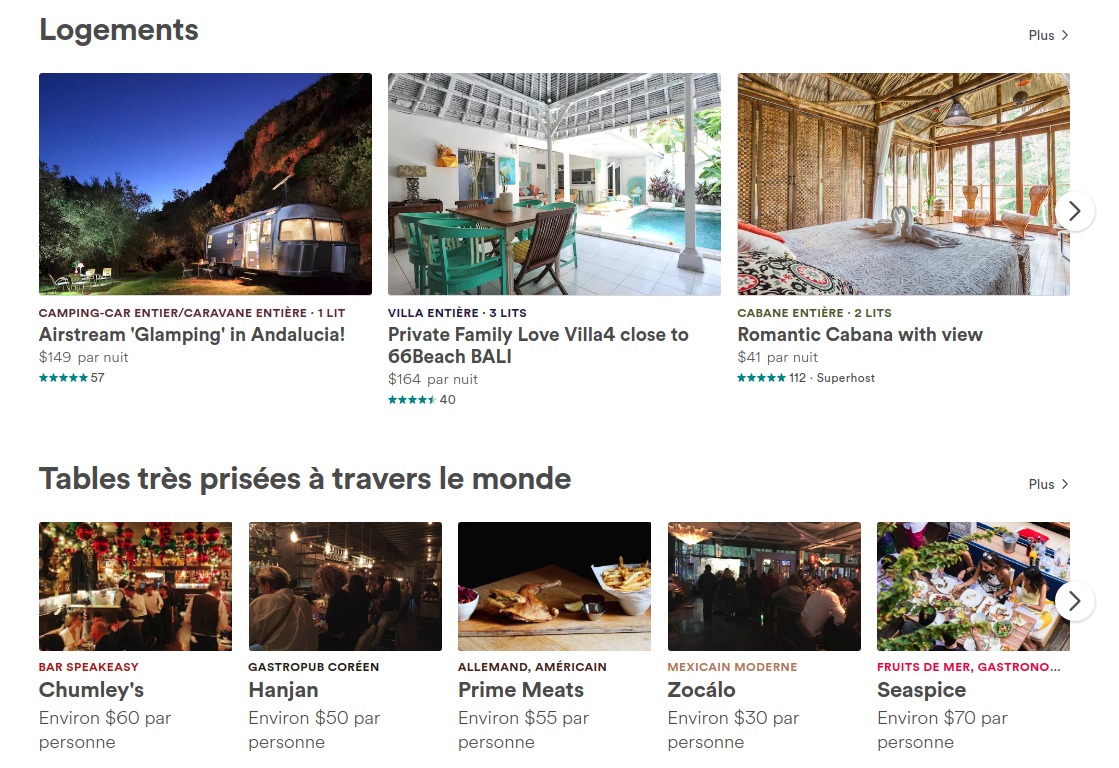
\includegraphics[width=17.5cm]{images/concurrent/airbnb1.png}
\end{center}
\caption{Accueil Airbnb}
\end{figure}

\paragraph{Les alternatives }
$ $\\Il s’agit de :
\begin{itemize}
\item[\textbullet] Tripping.com
\item[\textbullet] Booking.com
\item[\textbullet] Homeaway
\item[\textbullet] VRBO
\item[\textbullet] Trivago
\item[\textbullet] Outdoorsy
\item[\textbullet] Homestay
\item[\textbullet] Hotels.com
\item[\textbullet] Expedia
\item[\textbullet] Roomorama (ferme)
\item[\textbullet] Flipkey
\end{itemize}

\newpage
\begin{figure}[H]
\begin{center}

\includegraphics[width=17cm]{images/concurrent/airalt1.png}
\end{center}
\caption{Logos concurrents}
\end{figure}

Elles sont, pour la plupart nées suite à l’engouement autour de Airbnb. Ces plateformes proposent pêle-mêle : la location sur courte ou longue durée, la comparaison d’offres entre différentes plateformes, ...
\\Elles sont orientés exclusivement vers les marchés européen et américain.

\paragraph{Au Bénin : BeninMaison et BeninImmo}
$ $
\begin{figure}[H]
    \begin{minipage}[c]{.46\linewidth}
        \centering
        
\includegraphics[width=6.3cm]{images/concurrent/beninimmo2.png}
        \caption{Logo BeninImmo}
    \end{minipage}
    \hfill%
    \begin{minipage}[c]{.46\linewidth}
        \centering
        
\includegraphics[width=6.5cm]{images/concurrent/beninmaison2.png}
        \caption{Logo BeninMaison}
    \end{minipage}
\end{figure}

$ $
Ces plateformes  \footnote{https://beninmaison.com/, http://www.benin-immo.com/} proposent des services tel que:
\begin{itemize}
\item[\textbullet] Faire estimer un bien
\item[\textbullet] Mettre un bien en vente
\item[\textbullet] Mettre en location
\item[\textbullet] Acheter un bien immobilier
\item[\textbullet] Louer un logement
\item[\textbullet] Faire gérer son bien
\end{itemize}

\newpage
\begin{figure}[h]
\begin{center}
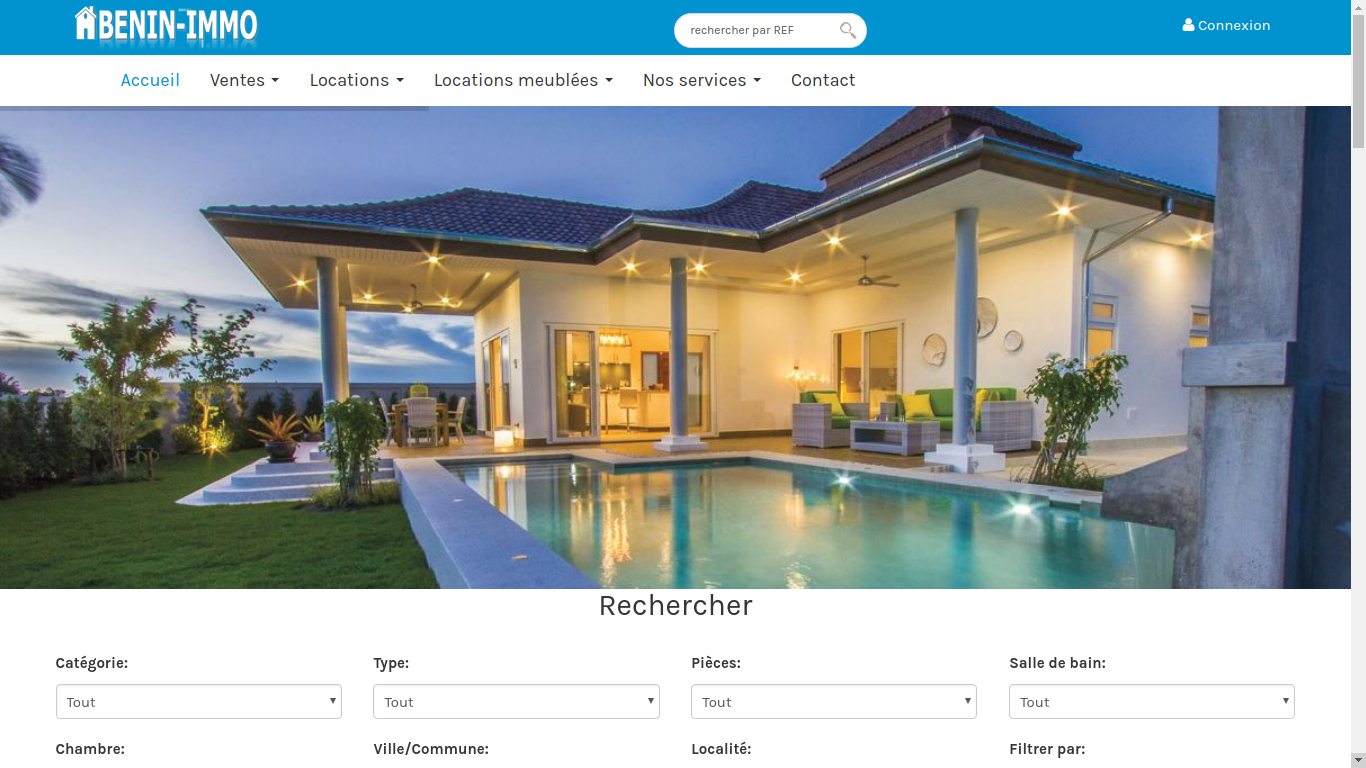
\includegraphics[width=17cm]{images/concurrent/beninimmo1.png}
\end{center}
\caption{Accueil BeninImmo}
\end{figure}

$\phantom{11111111111111111} $ $\phantom{11111111111111111}$
\begin{figure}[H]
\begin{center}

\includegraphics[width=17cm]{images/concurrent/beninmaison1.png}
\end{center}
\caption{Accueil BeninMaison}
\end{figure}

\newpage
\subsection{Intérêt de la solution par rapport aux existantes} 
Le leader du marché ainsi que ses concurrents occidentaux, orientent principalement leurs services vers les villes européennes et américaines. On note ainsi une très faible quantité d’offres provenant du Bénin.
\\Les plateformes béninoises quant à elles ont du mal à émerger. On citera entre autres comme problèmes observés :
\begin{itemize}
\item[\textbullet] la pauvreté de l’offre ;
\item[\textbullet] une UI\footnote{User Interface} très peu attrayante ;
\item[\textbullet] le manque ou l’absence de communication ;
\item[\textbullet] l’absence de moyen de paiement en ligne adapté ;
\subitem[\textbullet] Transactions internationales: Impossibilité de recevoir de l’argent sur un compte béninois via Paypal;
\subitem[\textbullet] Transactions locales : Faible bancarisation de la population locale, difficultés d’accès aux api MTN et MOOV mobile money;
\item[\textbullet] l’absence de location courte durée, et de la possibilité de louer une partie de son bien immobilier.
\end{itemize}

Avec notre application, les utilisateurs pourront réserver très rapidement un grand nombre de logements dans toutes les villes du Bénin. Ils pourront également vivre des expériences particulières avec un hôte de leur ville d'accueil. Une attention particulière sera accordée à l’interface d’utilisateur ainsi qu'à l'expérience d’utilisateur aussi bien sur la plateforme que sur le terrain par les commentaires et les notes.
\chapter{Analyse, conception, et choix techniques}

Pour conduire ce projet, nous avons opté pour la méthode de gestion de projet Scrum\footnote{Ken Schwaber et Jeff Sutherland, « Scrum Guide ». Scrum.org, 2013 p. 4.} qui est un schéma d’organisation de développement de produits complexes considérée comme une pratique agile; pratique qui implique au maximum le demandeur (client) et permet une grande réactivité à ses demandes. Scrum est défini comme un cadre de travail suivant un cycle de développement itératif, incrémental et adaptatif. S’appuyant sur le découpage d'un projet en boîtes de temps, nommées « sprints » pouvant durer entre quelques heures et un mois (avec une préférence pour deux semaines). Chaque sprint commence par une estimation suivie d'une planification opérationnelle et se termine par une démonstration de ce qui a été achevé.

\section{Analyse des besoins} 

L’analyse consiste à l’aboutissement de l’élaboration d’une solution technique à partir de l’étude des besoins. C’est la première phase du cycle de développement d’un logiciel. Elle sert à identifier les acteurs du système et leur associer chacun l’ensemble des actions avec lesquelles il intervient dans l’objectif de donner un résultat optimal et satisfaisant au client.

\subsection{Les besoins fonctionnels}

Les besoins fonctionnels répondent aux points précis du cahier de charges et sont donc requis par le client. Ils constituent le besoin primaire du client et définissent une fois résolu l’opérationnalité du système. Ainsi l’application doit permettre :

\paragraph{au visiteur de :}
\begin{itemize}
\item[\textbullet] gérer les informations de son compte
\item[\textbullet] consulter l’ensembles des offres d’appartements
\item[\textbullet] consulter l’ensembles des offres d'expériences
\item[\textbullet] réserver un appartement ou une partie d’appartement
\item[\textbullet] s’inscrire à une expérience
\item[\textbullet] prendre connaissances des tarifs
\item[\textbullet] payer une réservation
\item[\textbullet] reporter ou annuler une réservation dans les délai autorisés
\item[\textbullet] consulter l’historique de ses réservations et paiements
\item[\textbullet] demander le titre d’hôte
\item[\textbullet] poster un commentaire
\item[\textbullet] noter un d’hôte ou un logement
\item[\textbullet] recevoir des notifications et rappels
\end{itemize}


\paragraph{à l'hôte de :}
\begin{itemize}
\item[\textbullet] faire tout ce que peut faire un ‘’visiteur’’
\item[\textbullet] mettre en ligne des offres d’appartements ou de parties d’appartement
\item[\textbullet] proposer des expériences thématiques
\item[\textbullet] consulter son historique de réservations
\item[\textbullet] reporter ou annuler une réservation dans les délais autorisés
\item[\textbullet] noter un visiteur
\item[\textbullet] recevoir des paiements
\item[\textbullet] recevoir des notifications
\end{itemize} 

\paragraph{à l’administrateur}
\begin{itemize}
\item[\textbullet] d’accorder le titre d’hôte
\item[\textbullet] de retirer le titre d’hôte
\item[\textbullet] valider un commentaire
\item[\textbullet] d’envoyer les notifications
\item[\textbullet] d’interdire le report ou l’annulation d’une réservation à moins de 24 heures du jour
\end{itemize} 


\subsection{Les besoins non fonctionnels} 
Ces besoins sont soit des besoins optionnels soit des besoins/contraintes liés à l’implémentation. Ainsi, il faudra que l’application soit:
\begin{itemize}
\item[\textbullet] Sécurisée
\item[\textbullet] Dotés d’une bonne expérience utilisateur
\item[\textbullet] Performante
\end{itemize}

La version mobile devra être :
\\Compatible a tout système Android de version minimum 4.3
\\La version web, quand à elle, devra être:
\\Responsive design et compatible à la plupart des navigateurs
\newpage
\section{Choix de la méthode d'analyse} 

Pour la réalisation de notre application, nous avons besoin de gérer des données. De ce fait, l'utilisation d'une base de données est nécessaire. Selon Bouhaddaoui et al. (2010-2011)\footnote{Bouhaddaoui (M. Y.) et Tarek El Allam (M.) « Etude comparative sur les méthodes de modélisation: Comparatif UML - Merise ». Ecole Nationale Supérieure d'Ingénieurs de CAEN | 2010-2011.}, la conception d'une base de données n'est pas évidente car il faut réfléchir à l'ensemble de l'organisation que l'on doit mettre en place. La phase de conception nécessite des méthodes permettant de mettre en place un modèle sur lequel on va s'appuyer. Ce type de méthode est appelé analyse (Bouhaddaoui et al., 2010-2011).
\\$ $\\Il existe plusieurs méthodes d'analyse, notamment, Merise (Méthode d’Etude et de Réalisation Informatique par Sous-ensembles) et UML (Unified Modeling Language).
Selon Wikipedia (2017a)\footnote{Wikipedia, 2017a. « Merise (informatique) ». https://fr.wikipedia.org/wiki/Merise\_(informatique)}, Merise a été très utilisée dans les années 1970 et 1980. Merise est une méthode d’analyse et de conception de système d’information. Elle permet la modélisation des données et des traitements orientés bases de données (Wikipedia, 2017a). Selon Wikipedia (2017b)\footnote{Wikipedia, 2017b. « UML (informatique) ». https://fr.wikipedia.org/wiki/UML\_(informatique)} UML quant à lui est un langage de modélisation graphique à base de pictogrammes. Il est apparu dans le monde du génie logiciel, dans le cadre de la « conception orientée objet » et peut être appliqué à toutes sortes de systèmes ne se limitant pas au domaine informatique (Wikipedia, 2017b).
\\$ $\\Au niveau de l'abstraction des données, l’approche Merise permet de sérier les niveaux de préoccupations lors de la description ou de l'analyse du système suivant trois (03) niveaux :
\begin{itemize}
\item[\textbullet] le niveau conceptuel ;
\item[\textbullet] le niveau logique ;
\item[\textbullet] le niveau physique.
\end{itemize}

L'approche UML propose différentes notions (cas d'utilisation, paquetage, classe, composant, nœud) et différents diagrammes pour modéliser le système aux différents niveaux d'abstraction.
En ce qui concerne l'approche fonctionnelle, Merise propose une approche descendante où le système réel est décomposé en activités, elles-mêmes déclinées en fonctions. Les fonctions sont composées de règles de gestion, elles-mêmes regroupées en opérations. Ces règles de gestion au niveau conceptuel génèrent des modules décomposés en modules plus simples et ainsi de suite jusqu'à obtenir des modules élémentaires... Les limites d'une telle approche résident dans le fait que les modules sont difficilement extensibles et exploitables pour de nouveaux systèmes. Quant à UML, les fonctions cèdent la place aux cas d'utilisation qui permettent de situer les besoins de l'utilisateur dans le contexte réel. A chaque scénario correspond des diagrammes d'interaction entre les objets du système et non pas un diagramme de fonction.
\\$ $\\Une étude comparative des méthodes d’analyse réalisée par OSITEC-Consultants (2005) donne à UML un avantage absolu sur Merise du fait de son approche objet plus approfondie. De même que Bouhaddaoui et al. (2010-2011) qui vont plus loin en ajoutant qu’UML est international contrairement à Merise limité au monde francophone (Bouhaddaoui et al., 2010-2011).
Pour la suite de notre analyse, notre choix se portera donc sur UML pour sa précision, sa stabilité et son interopérabilité.

\newpage
\section{Analyse fonctionnelle et conceptuelle} 

\subsection{Analyse fonctionnelle} 
\subsubsection{Identification des acteurs et description} 
Un acteur peut consulter et/ou modifier directement l’état du système, en émettant et/ou en recevant des messages éventuellement porteurs de données. Il a une bonne connaissance des fonctionnalités du système. Il peut être soit un humain, un logiciel ou un automate. Dans le cadre de notre système nous avons retenu :
\begin{itemize}
\item[\textbullet] Le visiteur
\item[\textbullet] L’hôte
\item[\textbullet] L’administrateur
\end{itemize}

\subsubsection{Diagramme de cas d’utilisation} 
Le système est illustré par un diagramme de cas d’utilisation qui met en évidence les fonctions attendues du système (les cas d’utilisation), un environnement (les acteurs) et les relations entre cas d’utilisation et acteurs.

\subsubsubsection{Identification des cas d’utilisation}
Un cas d’utilisation est un concept de la méthode d’analyse UML. Il permet d’effectuer une délimitation du système et de décrire son comportement. Nous décrirons cinq (05) cas d’utilisation :
\begin{itemize}
\item[\textbullet] Mettre en location un appartement
\item[\textbullet] Proposer une expérience thématique
\item[\textbullet] Réserver un logement
\item[\textbullet] S’inscrire à une expérience
\item[\textbullet] Demander le titre d’hôte
\end{itemize}

\subsubsubsection{Description textuelle des cas d'utilisation}
Pour détailler la dynamique d'un cas d’utilisation, la procédure la plus évidente consiste à recenser de façon textuelle toutes les interactions entre les acteurs et le système. Le cas d’utilisation doit avoir un début et une fin clairement identifiés. La description d’un cas d’utilisation permet de :
\begin{itemize}
\item[\textbullet] clarifier le déroulement de la fonctionnalité ;
\item[\textbullet] décrire la chronologie des actions qui devront être réalisées ;
\item[\textbullet] identifier les parties redondantes pour en déduire des cas d’utilisation plus précises qui seront utilisées par inclusion, extension ou généralisation/spécialisation ;
\item[\textbullet] indiquer d’éventuelles contraintes déjà connues et dont nous devrons tenir compte lors de la réalisation de l'application.
\end{itemize}

\newpage

\paragraph{a - Cas d'utilisation : Demander le titre d’hôte} 
$ $\\$ $\\\underline{\textbf{Acteurs}} : Visiteur
\\\underline{\textbf{Description}}  : Permet à l’utilisateur d’obtenir le statut d'hôte et donc de pouvoir proposer des logements ou des expériences
\\\underline{\textbf{Pré-condition}} : L'utilisateur est connecté au système d’information.
\\\underline{\textbf{Démarrage}} : L’utilisateur lance l’application.
\\\underline{\textbf{Scénario nominal}} :

\begin{table}[H]
\begin{center}
\begin{tabular}{|p{8cm}|p{8cm}|}
\hline
Visiteur & Système\\
\hline
1- L’utilisateur s’authentifie & $ $\\
\hline	
2- L’utilisateur arrive sur l’interface principale & $ $\\
\hline 	
3- Clique sur le bouton Devenir Hôte & 4- Affiche le formulaire de demande\\
\hline
5- Saisi les informations demandées et joint une copie scannée de sa carte d'identité & $ $\\
\hline	
6- Remplit les informations de son moyen de paiement afin de pouvoir recevoir les paiements depuis l’application & 6- Délivre une autorisation temporaire en attendant que les données soient vérifiées\\
\hline
\end{tabular}
\caption{Scénario nominal - Cas d'utilisation : Demander le titre d'hôte}
\end{center}
\end{table}

\begin{flushleft}
 \underline{\textbf{Post condition}} : L’utilisateur peut désormais proposer des logements et des expériences.
\\\underline{\textbf{Scénario alternatif}}:
\textbf{A1} : Données saisies invalides ou incomplètes
\\L'enchaînement A1 démarre au point 5 du scénario nominal.
\\6- Le système indique que les informations saisies sont erronées. Le cas d’utilisation se termine en échec.
\end{flushleft}

\newpage
\paragraph{b - Cas d'utilisation : Mettre en location un appartement} 
$ $\\$ $\\\underline{\textbf{Acteurs}} : Hôte
\\\underline{\textbf{Description}} : Permet à l'hôte de proposer des logements.
\\\underline{\textbf{Pré-conditions}} : L'utilisateur est connecté au système d’information. L'utilisateur est un hôte.
\\\underline{\textbf{Démarrage}}: L’utilisateur lance l’application.
\\\underline{\textbf{Scénario nominal}} :

\begin{table}[H]
\begin{center}
\begin{tabular}{|p{8cm}|p{8cm}|}
\hline
Hôte & Système\\
\hline
1- L’utilisateur s’authentifie & $ $\\
\hline
2- L’utilisateur arrive sur l’interface principale  & $ $\\	
\hline
3- Clique sur le bouton Publier un logement & 4- Affiche le formulaire d’information n1 (Lits, salles de bain, équipements)\\
\hline
5- L'hôte indique le type de logement, ainsi que, le nombre maximal de visiteurs qu’il souhaite accueillir dans son logement & $ $\\
\hline
6- L'hôte indique le nombre de chambres, de lits, de salles de bain, ainsi que les équipements (serviettes, draps, savon, Wi-Fi, télévision, climatisation) que les visiteurs peuvent utiliser & $ $\\
\hline
7- L'hôte indique la localisation précise de son logement : Numéro et nom de la rue, Ville, Département, emplacement précis sur la carte & 8- Récupère la localisation de l’appareil de l’utilisateur et affiche une carte Google Map\\
\hline
$ $ & 9- Affiche le formulaire d’information n2 (Photos, description)\\
\hline
10- L'hôte renseigne le nom et met en ligne des photos ainsi qu’une description de son logement	 & $ $\\
\hline
$ $ & 11- Affiche le formulaire d’information n3 (Accueil)\\
\hline
12- L'hôte établit un règlement intérieur & $ $\\
\hline
13- L'hôte établit un calendrier de disponibilité	 & $ $\\
\hline
14- L'hôte fixe un prix pour son logement & 15- Confirme la mise en location du logement\\
\hline
\end{tabular}
\caption{Scénario nominal - Cas d'utilisation : Mettre en location un appartement}
\end{center}
\end{table}


\begin{flushleft}
{\underline{\textbf{Post condition}}} : L’utilisateur peut désormais recevoir des offres de réservation pour son logement.
\\\underline{\textbf{Scénario alternatif}} :
\\\textbf{A1} : La localisation précise n’a pu être obtenue avec succès.
\\L'enchaînement A1 démarre au point 7 du scénario nominal.
\\8- Le système indique que les informations saisies sont erronées. Le scénario nominal reprend au point 7.
\end{flushleft}

\newpage
\paragraph{c - Cas d'utilisation : Proposer une expérience thématique} 
$ $\\$ $\\\underline{\textbf{Acteurs}} : Hôte
\\\underline{\textbf{Description}} : Permet à l'hôte de créer des expériences.
\\\underline{\textbf{Pré-conditions}} : L'utilisateur est connecté au système d’information. L’utilisateur est un hôte.
\\\underline{\textbf{Démarrage}}: L’utilisateur lance l’application.
\\\underline{\textbf{Scénario nominal}} :

\begin{table}[H]
\begin{center}
\begin{tabular}{|p{8cm}|p{8cm}|}
\hline
Hôte & Système\\
\hline
1- L’utilisateur s’authentifie & $ $\\
\hline
2- L’utilisateur arrive sur l’interface principale & $ $\\
\hline	
3- Clique sur le bouton Créer une expérience & 4- Affiche le formulaire d’information\\
\hline
5- L'hôte remplit et soumet le formulaire conformement aux critères de qualité établis & 6- La réponse est prise en compte et sera traitée ultérieurement conformément aux critères de qualité établis\\
\hline
\end{tabular}
\caption{Scénario nominal - Cas d'utilisation : Proposer une expérience thématique}
\end{center}
\end{table}
\begin{flushleft}
\underline{\textbf{Post condition}} : L’utilisateur est notifié lorsque sa demande est acceptée. Il peut désormais recevoir des offres d’inscription pour son expérience thématique.
\end{flushleft}

\paragraph{d - Cas d'utilisation : Réserver un logement} 
$ $\\$ $\\\underline{\textbf{Acteurs}} : Visiteur
\\\underline{\textbf{Description}} : Permet à l’utilisateur de réserver un logement de son choix.
\\\underline{\textbf{Pré-conditions}} : L'utilisateur est connecté au système d’information.
\\\underline{\textbf{Démarrage}} : L’utilisateur lance l’application.
\\\underline{\textbf{Scénario nominal}} :

\begin{table}[H]
\begin{center}
\begin{tabular}{|p{8cm}|p{8cm}|}
\hline
Visiteur & Système\\
\hline
1- L’utilisateur s’authentifie	& $ $\\
\hline
2- L’utilisateur arrive sur l’interface principale & $ $\\
\hline	
3- Recherche un logement en renseignant sa ville de destination et des informations complémentaires telles que la nature du logement désiré et le nombre de personnes à loger & 4- Affiche la liste des logement correspondant a la recherche de l'utilisateur\\
\hline
5- Choisi un logement dans la liste affiche & 6- Affiche la fiche descriptive du logement\\
\hline
7- Renseigne sa date d'arrivée, date de départ et commence la procédure de réservation & 8- Affiche le prix correspondant aux options choisies\\
\hline
9- Renseigne un moyen de paiement valide (Carte visa, Paypal) & 10- Envoie la réponse l'hôte\\
\hline
11- Valide le paiement & 12- Informe l'hôte et met à jour le calendrier de disponibilité du logement\\
\hline
\end{tabular}
\caption{Scénario nominal - Cas d'utilisation : Réserver un logement}
\end{center}
\end{table}

\begin{flushleft}
\underline{\textbf{Post condition}} : L’utilisateur prends contact avec l'hôte afin de disposer du logement réservé.
\\\underline{\textbf{Scénario alternatif}} :
\\\textbf{A1} : Données de paiement saisies invalides ou incomplètes
\\L'enchaînement A1 démarre au point 9 du scénario nominal.
\\10- Le système indique que les informations saisies sont erronées. Le cas d’utilisation se termine en échec.
\\$ $\\\textbf{A2} : L'hôte rejette la demande de réservation
\\L'enchaînement A2 démarre au point 10 du scénario nominal.
\\11- Le visiteur ne peut continuer la procédure de réservation. Le cas d’utilisation se termine en échec.
\end{flushleft}

\paragraph{e - Cas d'utilisation : S’inscrire à une expérience}
$ $\\$ $\\\underline{\textbf{Acteurs}} : Visiteur
\\\underline{\textbf{Description}} : Permet à l’utilisateur de s’inscrire à une expérience thématique.
\\\underline{\textbf{Pré-conditions}} : L'utilisateur est connecté au système d’information.
\\\underline{\textbf{Démarrage}} : L’utilisateur lance l’application.
\\\underline{\textbf{Scénario nominal}} :

\begin{table}[h]
\begin{center}
\begin{tabular}{|p{8cm}|p{8cm}|}
\hline
Visiteur & Système\\
\hline
1- L’utilisateur s’authentifie & $ $\\
\hline	
2- L’utilisateur arrive sur l’interface principale & $ $\\
\hline 	
3- Recherche une expérience en renseignant sa ville de destination et des informations complémentaires telles que la thématique voulue & 4- Affiche la liste des expériences correspondant a la recherche de l'utilisateur\\
\hline
5- Choisit une expérience dans la liste affiche & 6- Affiche la fiche descriptive de l'expérience\\
\hline
7- Renseigne sa date de réservation et le nombre de participants qu’il voudrait inscrire & 8- Affiche le prix correspondant aux options choisies\\
\hline
9- Renseigne un moyen de paiement valide (Carte visa, Paypal) & $ $\\
\hline
\end{tabular}
\caption{Scénario nominal - Cas d'utilisation : S’inscrire à une expérience}
\end{center}
\end{table}
\begin{flushleft}
\underline{\textbf{Post condition}} : La réservation est effectuée. Le visiteur peut participer à l'activité
\end{flushleft}

\newpage
\subsubsubsection{Présentation du diagramme de cas d'utilisation}
Le diagramme de cas d'utilisation retenu après analyse se présente comme suit :
\begin{figure}[H]
	\begin{center}
		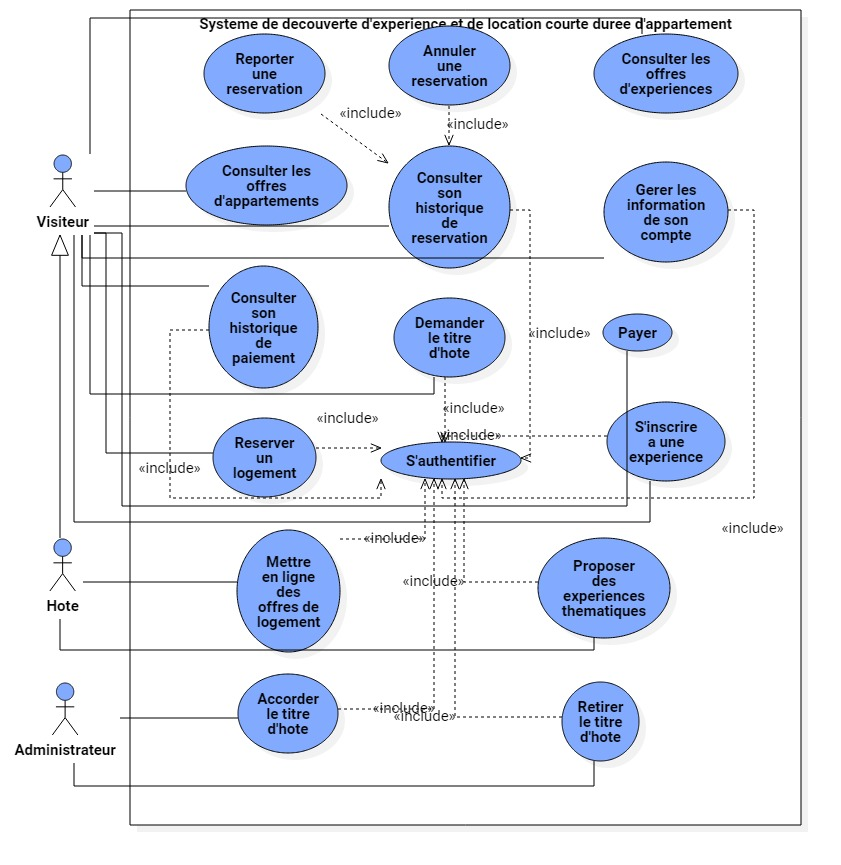
\includegraphics[width=18cm]{images/uml/UseCaseDiagram.jpg}
	\end{center}
	\caption{Diagramme de cas d'utilisation}
\end{figure}


\subsection{Analyse conceptuelle} 
\subsubsection{Diagramme des classes} 
Le diagramme des classes est considéré comme le plus important des diagrammes de la modélisation et de la structure interne du système. Il permet de fournir une représentation abstraite des objets du système qui vont interagir ensemble pour réaliser les cas d’utilisation.
\\$ $\\Notre étude a abouti au diagramme de classes suivant :
\begin{figure}[H]
	\begin{center}
		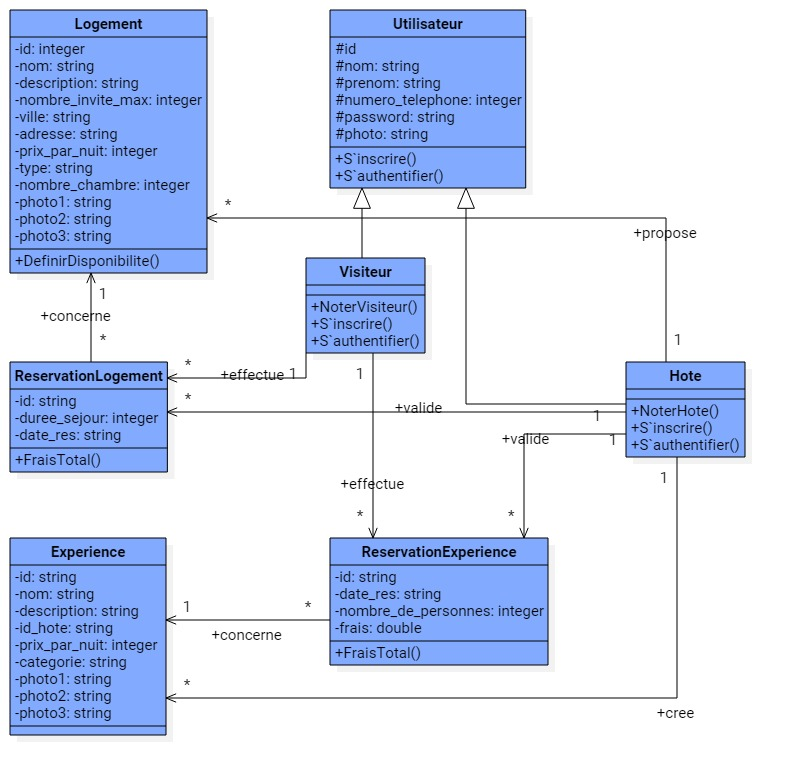
\includegraphics[width=18cm]{images/uml/ClassDiagram.jpg}
	\end{center}
	\caption{Diagramme des classes}
\end{figure}

\subsubsection{Diagramme de séquence} 
UML fournit les diagrammes d’interaction qui permettent de représenter la façon dont les objets réagissent via des messages. Il en existe deux (02) grands types : les diagrammes de séquence et les diagrammes de communication. Cependant, dans le cadre de notre domaine d’étude, nous allons présenter uniquement le diagramme de séquence.
\\Les diagrammes de séquences sont importants pour les raisons suivantes:
\begin{itemize}
\item[•] Ils permettent d'illustrer et vérifier le comportement d’un ensemble d’objet (système ou sous- système) ;
\item[•] Ils aident à la découverte des objets du système ;
\item[•] Ils aident à la découverte des méthodes des objets.
\end{itemize}

Nous allons présenter quelques diagrammes de séquences :
\begin{figure}[H]
	\begin{center}
		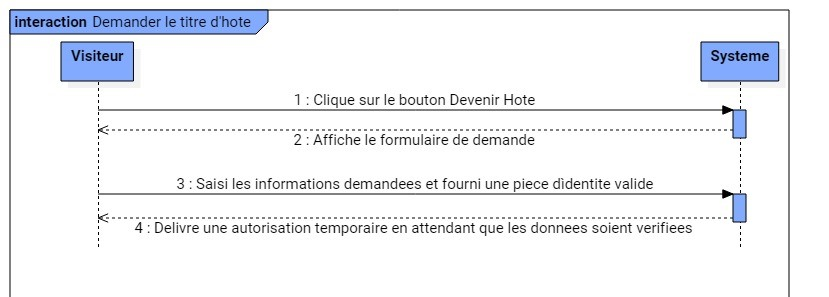
\includegraphics[width=18cm]{images/uml/SeqDemanderTitreHote.jpg}
	\end{center}
	\caption{Diagramme de séquence : Demander le titre d’hote}
\end{figure}
$ $
\begin{figure}[H]
	\begin{center}
		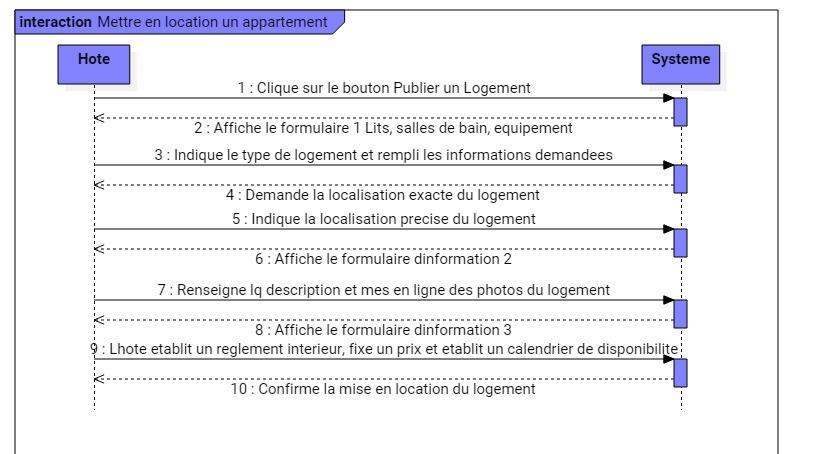
\includegraphics[width=18cm]{images/uml/SeqMettreLocationAppartement.jpg}
	\end{center}
	\caption{Diagramme de séquence : Mettre en location un appartement}
\end{figure}
$ $
\begin{figure}[H]
	\begin{center}
		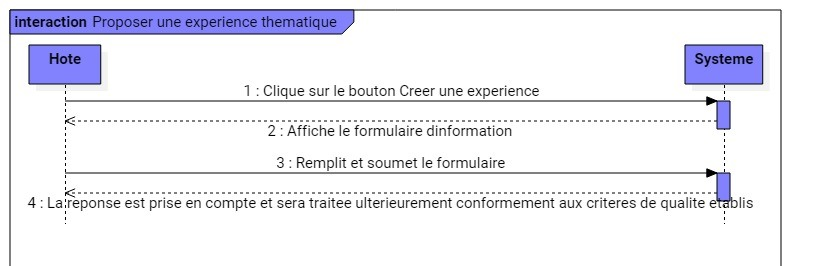
\includegraphics[width=18cm]{images/uml/SeqProposerExperienceThematique.jpg}
	\end{center}
	\caption{Diagramme de séquence : Proposer une expérience thématique}
\end{figure}
$ $
\begin{figure}[H]
	\begin{center}
		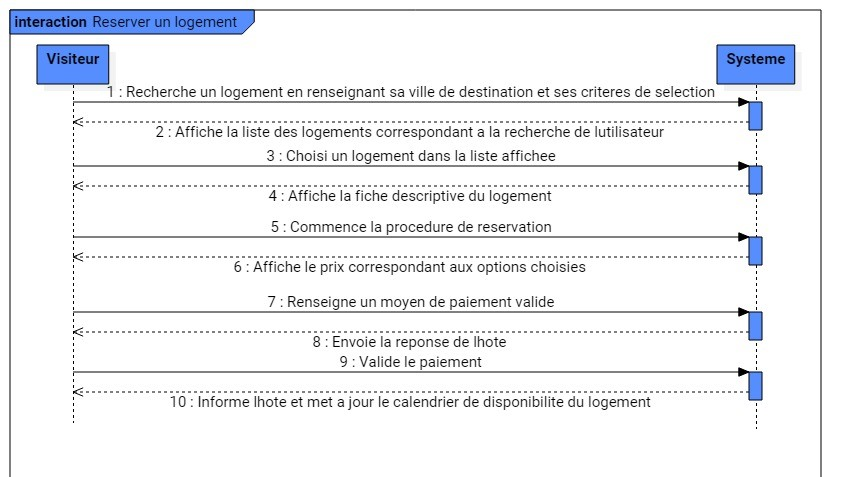
\includegraphics[width=18cm]{images/uml/SeqReserverLogement.jpg}
	\end{center}
	\caption{Diagramme de séquence : Réserver un logement}
\end{figure}
$ $
\begin{figure}[H]
	\begin{center}
		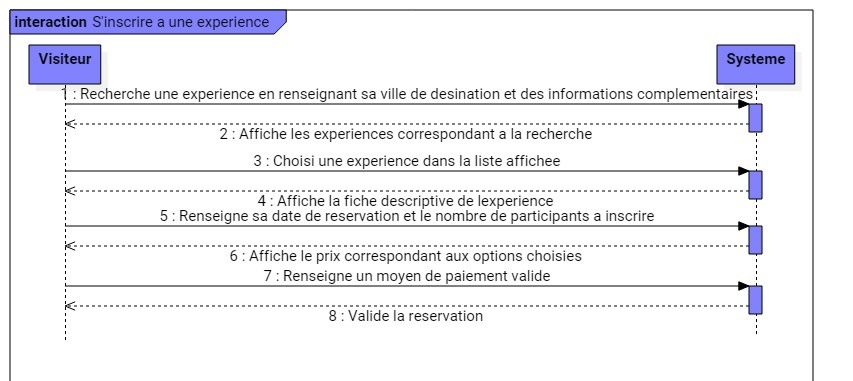
\includegraphics[width=18cm]{images/uml/SeqInscrireExperience.jpg}
	\end{center}
	\caption{Diagramme de séquence : S’inscrire à une expérience}
\end{figure}

\section{Choix des outils d'implémentation}
Cette partie présentera ensemble de technologies et outils que nous avons
mis en oeuvre dans l’implémentation de notre système.

\subsection{Architecture du système} 
Au vue du cahier des charges nous devrions produire au minimum deux applications qui partagent un ensemble d’informations mais pour différents publics. En effet nous devons récupérer un certains nombres d’informations du système de façon sécurisée et les distribuer aussi de façons contrôlée à la fois entre l’application mobile sur android et l’application web. De même ces deux applications devraient échanger entre elle un ensemble d’informations et de fonctionnalités propres au système à concevoir. 

Pour cela il faudrait déjà dans un premier temps qu’elles (les applications) partagent une base de données commune (centralisée), mais aussi un point d’entré commun pour accéder à cette base de données. Ce besoin nous amène donc à concevoir une interface de programmation au dessus du système d’information. Une architecture client serveur 3-tiers se décerne donc comme solution architecturale à notre cas. Cette dernière sépare l’application en 3 niveaux à savoir :

\paragraph{Niveau 1:} La couche présentation (ou affichage si l'on souhaite) associée au client qui de fait est dit "léger" dans la mesure où il n'assume aucune fonction de traitement.

\paragraph{Niveau 2:} La couche fonctionnelle liée au serveur, comprend le serveur d'applications ou middleware qui dans notre cas est un serveur Web interagissant avec la base de données et les clients.

\paragraph{Niveau 3:} La couche de données liée au serveur de base de données (SGBD).

Au coeur de cette architecture un composant dénommé API pour Application Programming Interface soit
Interface de programmation applicative devra fournir sous forme de services les
fonctionnalités qui ont trait à la logique du métier pour toutes nos applications clientes à conditions d'être autorisée. Ainsi toutes les fonctionnalités métier citées dans la partie application mobile et Application web doivent être développée au niveau de cette API. Les applications tierces à savoir l’application mobile et l’application web ne seront que de simple consommatrice de ces services.
De façon architecturale notre système ressemblerait ceci :
$ $
\begin{figure}[H]
	\begin{center}
		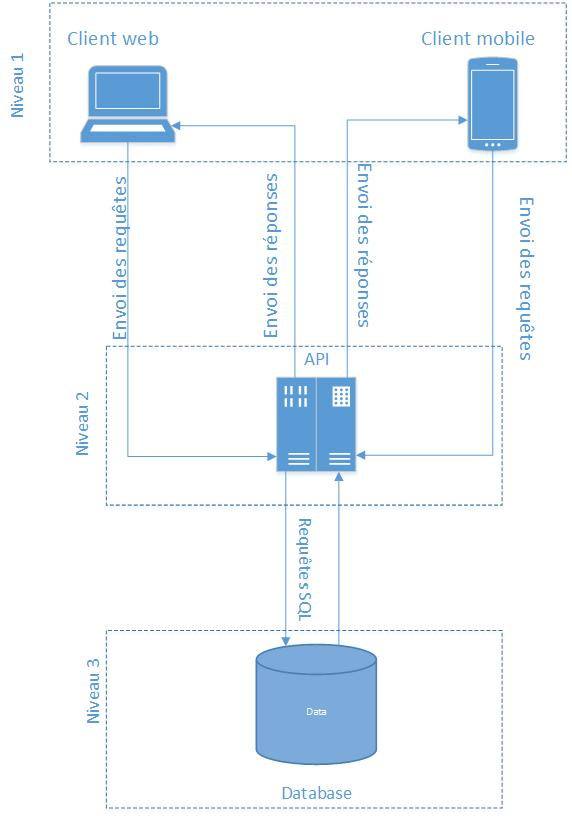
\includegraphics[width=14cm]{images/techno/3tiers.jpg}
	\end{center}
	\caption{Architecture du système}
\end{figure}
$ $
\subsection{Couche présentation} 
\subsubsection{Client Web}
\begin{figure}[H]
	\begin{center}
		
\includegraphics[width=14cm]{images/techno/mern.png}
	\end{center}
	\caption{MongoDB - ExpressJs - React - NodeJs}
\end{figure}
$ $\\Au niveau du client web nous utilisons la pile logicielle JavaScript moderne avec en son coeur le framework React en plus des langages classiques HTML et CSS respectivement dans leurs versions 5 et 3.
\begin{figure}[H]
	\begin{center}
		
\includegraphics[width=10cm]{images/techno/jsarchi.png}
	\end{center}
	\caption{Moderne Stack Javascript}
\end{figure}

\paragraph{React.js} 
$ $\\Plus qu'une bibliothèque ou un framework, React est un paradigme de programmation d'interfaces utilisateurs, qui permet d'adresser de nombreuses plateformes, avec toujours du code React "standard".
\\Théoriquement, une application codée en React est capable de produire n'importe quel output, par exemple du HTML pour le web, du natif avec react-native, du WebGL, du terminal, de la musique...

\newpage
\subsubsection{Client Mobile}
$ $\\Le service a été pensé pour être accessible via un terminal mobile, indépendamment de la plateforme. Nous avons donc opté pour la réalisation d’une application mobile. Par conséquent il a fallu opérer un choix entre développement natif et hybride.
\\$ $\\Les applications natives, applications conçues spécifiquement pour un système d'exploitation, ont l'avantage d'offrir une expérience utilisateur et des performances optimisées pour leur plateforme spécifique. Cependant, la concentration sur une seule plateforme représente justement leur principal inconvénient. En effet, rendre la même application disponible sur une autre plateforme nécessite de la réécrire dans un langage spécifique à la plateforme choisie : Java ou Kotlin pour Android, Objective-C ou Swift pour iOS.
\\$ $\\Les applications hybrides quant à elles, se basent sur un même jeu de standards indépendamment de la plateforme choisie. Porter une application hybride vers plusieurs plateformes implique simplement de recompiler le même code source pour chacune d'elles. En contrepartie, elles offrent des performances moindres sur les terminaux les plus anciens et un accès limité à certaines fonctionnalités natives. Le souci de performance a longtemps limité leur pertinence. Cependant, de récentes avancées ont élargi leur champ de possibilités : Géo localisation, performances améliorées, accès à la caméra et au microphone, envoi de notifications, etc.
\\$ $\\Ces facteurs ont donc motivé le choix du développement hybride : Ionic, pour notre application client.
\subsubsection{Gestion de versions}
Nous terminerons cette partie par la présentation de Git un outil qui a été au cœur de notre travail de développement. Pour une bonne continuité dans l’implémentation et pour prévenir le risque que survienne un problème dans l’implémentation ou une perte des données du disque dur, nous avons besoin d’un gestionnaire de version. Notre choix s'est donc porté sur Git qui est un logiciel de gestion de version décentralisé. C'est un logiciel libre créé par Linus Torvalds, auteur du noyau Linux. En 2017, il s’agit du logiciel de gestion de versions le plus populaire qui est utilisé par plus de douze millions de développeurs (d’après Github). Comme Dépôt en ligne, nous avons utilisé la version communautaire de Gitlab avec des dépôts privés.

\subsection{Couche fonctionnelle} 
Elle permet d’assurer la transmission de la couche données vers la couche présentation, et inversement. Pour cela, il est fait recours à un middleware, sous la forme d’un web service. De nos jours, le standard REST est le plus répandu pour le développement des web services.
\\$ $\\REST (Representational State Transfer) ou RESTful est un style d’architecture permettant de construire des applications (Web, Intranet, Web Service). Il s’agit d’un ensemble de conventions et de bonnes pratiques à respecter et non d’une technologie à part entière. L’architecture REST utilise les spécifications originelles du protocole HTTP, plutôt que de réinventer une surcouche (comme le font SOAP ou XML-RPC par exemple). Une API compatible REST ou « RESTful » est une interface de programmation d'application qui fait appel à des requêtes HTTP. Dans cette architecture REST nous avons choisis le JSON comme format d'achat de données pour ça syntaxe souple qui favorise la rapidité des échanges.
\newpage
Nous avons choisi Node.js pour la réalisation de notre API REST. En effet, jusqu'ici, le JavaScript avait toujours été utilisé du côté du client, c'est-à-dire du côté du visiteur qui navigue sur notre site. Le navigateur web du visiteur (Firefox, Chrome, IE...) exécute le code JavaScript et effectue des actions sur la page web. Node.js nous permet d'utiliser le langage JavaScript sur le serveur.
\\$ $\\Au cœur de l’architecture node.js on retrouve des opérations IO non bloquantes, que ce soit à propos des interactions réseaux, ou de toutes les autres formes d’entrées/sorties, notamment le système de fichiers et les différentes bases de données aujourd’hui disponibles. C’est cet ensemble de bibliothèques IO non bloquantes, HTTP et autres protocoles de plus bas niveau (tcp, udp) que Node introduit au dessus du moteur JavaScript v8.
\\$ $\\Cet usage optimisé du matériel nous permet d’utiliser des serveurs plus léger sans avoir à sacrifier la performance aux yeux de l’utilisateur et ainsi traiter des milliers de requêtes simultanées, avec une empreinte mémoire faible.

\subsection{Couche données} 
Un Système de Gestion de Base de Données (SGBD) est un logiciel système destiné à stocker et à partager des informations dans une base de données, en garantissant la qualité, la pérennité et la confidentialité des informations, tout en cachant la complexité des opérations. Il permet d'inscrire, de retrouver, de modifier, de trier, de transformer ou d'imprimer les informations de la base de données.

\paragraph{MySQL} 
$ $\\MySQL est un serveur de bases de données relationnelles SQL développé dans un souci de performances élevées en lecture, ce qui signifie qu'il est davantage orienté vers le service de données déjà en place que vers celui de mises à jour fréquentes et fortement sécurisées. Il est multi-thread et multi-utilisateur. C'est un logiciel libre, open source, développé sous double licence selon qu'il est distribué avec un produit libre ou avec un produit propriétaire.

\paragraph{PostgreSQL}
 $ $\\PostgreSQL est un système de gestion de bases de données relationnel robuste et puissant, aux fonctionnalités riches et avancées, capable de manipuler en toute fiabilité de gros volumes de données, même dans des situations critiques. Il est de type SQL et extrêmement respectueux des standards, se conformant au plus près à la norme ANSI-SQL 2008.

\paragraph{MongoDB}
$ $\\MongoDB (de l'anglais humongous qui peut être traduit par « énorme ») est un système de gestion de base de données orientée documents, répartissable sur un nombre quelconque d'ordinateurs et ne nécessitant pas de schéma prédéfini des données. MongoDB est développé depuis 2007 par MongoDB et fait partie de la mouvance NoSQL (Not Only SQL). MongoDB permet de manipuler des objets structurés au format BSON (JSON binaire), sans schéma prédéterminé. En d'autres termes, des clés peuvent être ajoutées à tout moment « à la volée », sans reconfiguration de la base.

\paragraph{Choix}:
$ $\\Notre choix s’est porté sur MongoDB. La raison principale de notre orientation est que c’est le SGBD que nous avons eu a utiliser durant notre stage aussi bien en développement qu’en production\footnote{www.mongomanager.space}. De plus, pour stocker les données de traitement de notre système nous avons utilisé une base de données NoSQL “Not only SQL” pour sa scalabilité horizontale\footnote{La scalabilité verticale implique d’augmenter les ressources de calcul de chaque serveur composant l’infrastructure tandis que la scalabilité horizontale, consiste à multiplier les nœuds de calcul au niveau le plus bas de l’infrastructure et à configurer les logiciels de middleware pour qu’ils s’exécutent sur de multiples hôtes redondants de manière à assurer une répartition optimale de la charge (load-balancing)} et sa capacité à permettre la gestion de volumes de données importants. NoSQL permet également des traitements plus rapides pour certains types d'applications.


\section{Sécurité de l’application}
Le système que nous avons développé traite des informations sensibles : les données personnelles et banquaires des utilisateurs. A partir du moment ou nous faisons transiter ces informations
entre différents réseaux et interconnectant différentes applications nous devrions
prendre des mesures sécuritaire pour réduire autant que possible les failles de
sécurité.
$ $\\Nous classons ci-dessous les mesures que nous avons adoptées en fonctions
des principes de sécurité informatique :
\subsection{La confidentialité}
La confidentialité est le fait de s’assurer qu’une information est accessible
uniquement par les entités qui ont le droit d’accéder à celle-ci.
Le système que nous avons développé intègre cet aspect de la sécurité à deux
niveaux :
\begin{itemize}
	\item[\textbullet] Dans un premier temps nous avons installer un certificat ssl de 2048 bits
	qui nous permet de sécuriser toutes les communications utilisant le
	protocole tcp/ip.
	\item[\textbullet] Dans un second temps un système de gestion de rôle et de droit intégré
	nous permet de respecter la confidentialité des données dans chaque sous
	système. En effet chaque utilisateur appartient à un groupe
	d’utilisateurs donné et pour chaque groupe seulement un ensemble
	d’actions bien définies sont possibles.
\end{itemize}
\subsection{L’Intégrité}
L’intégrité s’assure que la donnée reste toujours intègre c’est-à-dire
qu’elle n’a pas été modifiée par un tiers non autorisé. Cet principe de sécurité
est pris en compte par la mise en place d’un certificat ssl sur le serveur
d’applications.
\subsection{La disponibilité}
La disponibilité est le fait de s’assurer que l’information soit toujours
disponible peu importe le moment choisit.
$ $\\Elle a été assurée en partie par l'infrastructure mise en place comme des
serveur de redondance mais aussi par la virtualisation des ressources et des
applications qui ont été déployées. Aussi une gestion de la montée en charge a
été prévue mais n’a pas été implémenté.
\subsection{L’Authenticité}
Au sein d’un système d’information, il est important de vérifier
l’authenticité de chaque ressource. Cela est possible grâce au mécanisme
d’authentification, qui permet de prouver l’identité d’une personne via le
processus d’identification.
$ $\\A notre niveau nous avons mis cela en place par une forte authentification
à deux niveaux. Dans un premier temps avant de faire appel à une quelconque
URI il faudrait être authentifié avec un couple d’identifiant comme service tiers
de confiance. Donc nos applications clientes s’authentifient avant de demander
un quelconque service au Backend. Après être autorisé les applications clientes
ont le devoir d’authentifier leurs utilisateurs avant de pouvoir faire une
opération (lecture ou écriture) mettant en relation un utilisateur du système.
$ $\\Bien qu’ayant installé un certificat sur le serveur nous évitons de faire
circuler les paramètres de connexion de l'utilisateur. En lieu et place nous avons
utilisé un jeton qui est une longue chaîne de caractères générée et encryptée
automatiquement lors de l’authentification de l’utilisateur. C’est désormais cette
clé renouvelable et ayant une durée de vie limitée qui est désormais envoyé
conjointement avec les requêtes pour authentifier l’utilisateur. Toute requêtes ne
contenant pas de jeton ou contenant des jetons invalide sont automatiquement
rejetées.
\subsection{Non-répudiation}
La non-répudiation se base sur un principe simple : une entité ne peut nier
son implication dans une action à laquelle il a participé.
$ $\\Dans notre cas la non-répudiation peut être atteinte seulement en utilisant la
technologie du certificat numérique avec un chiffrement asymétrique.
\subsection{Imputabilité}
Il s’agit des techniques mises en oeuvres pour assurer la traçabilité des actions
d’un individu sur un système. Nous avons mis en place cette traçabilité en
journalisation toutes les actions menées sur les objets du système.
\chapter{Réalisation de l'application}

\section{Captures d'ecran}
\subsection{Client Mobile}
L'application se présente en plusieurs parties. Nous distinguons le panel d’authentification qui permet
à l’utilisateur de s’inscrire lors de la première utilisation et de se connecter afin d’accéder aux
autres modules de l’application. Les interfaces ci-après la présentent :
\begin{figure}[h]
    \begin{minipage}[c]{.46\linewidth}
        \centering
        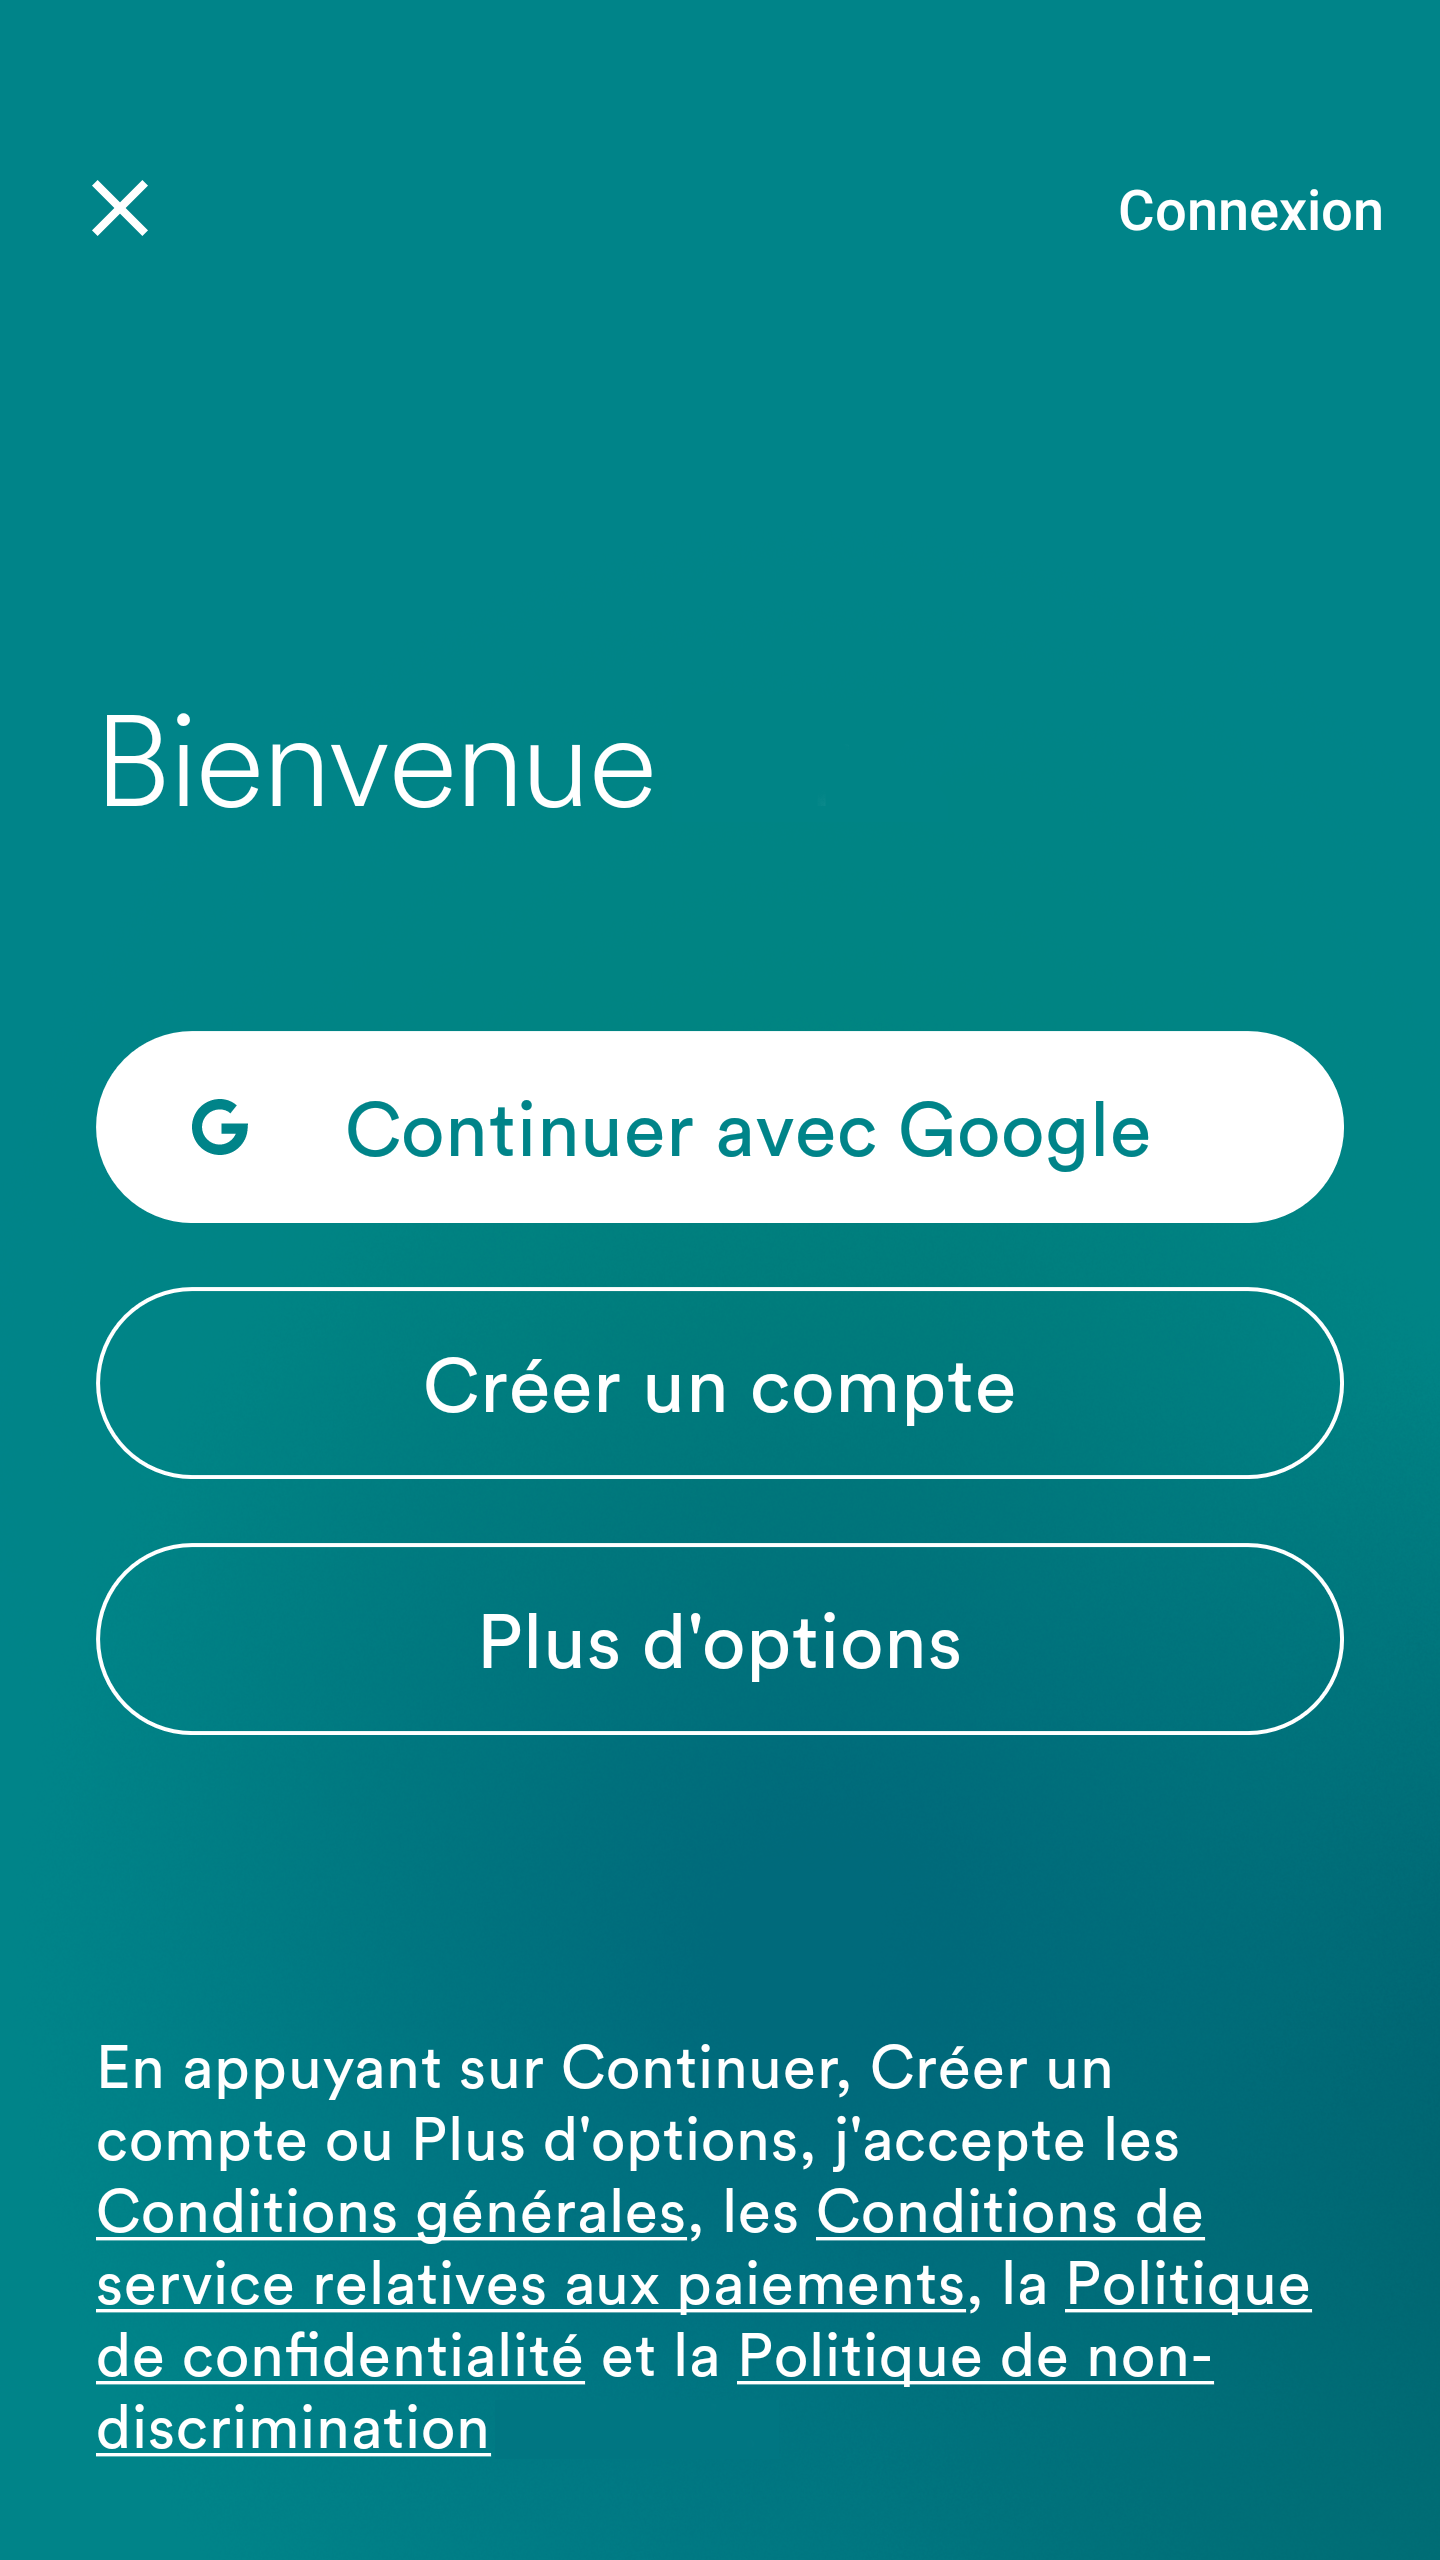
\includegraphics[width=6.5cm]{images/screen/mobile/1.png}
        \caption{Accueil - Inscription}
    \end{minipage}
    \hfill%
    \begin{minipage}[c]{.46\linewidth}
        \centering
        
\includegraphics[width=6.5cm]{images/screen/mobile/2.png}
        \caption{Nom - Inscription}
    \end{minipage}
\end{figure}
$ $
\begin{figure}[h]
    \begin{minipage}[c]{.46\linewidth}
        \centering
        
\includegraphics[width=6.5cm]{images/screen/mobile/3.png}
        \caption{Mail - Inscription}
    \end{minipage}
    \hfill%
    \begin{minipage}[c]{.46\linewidth}
        \centering
        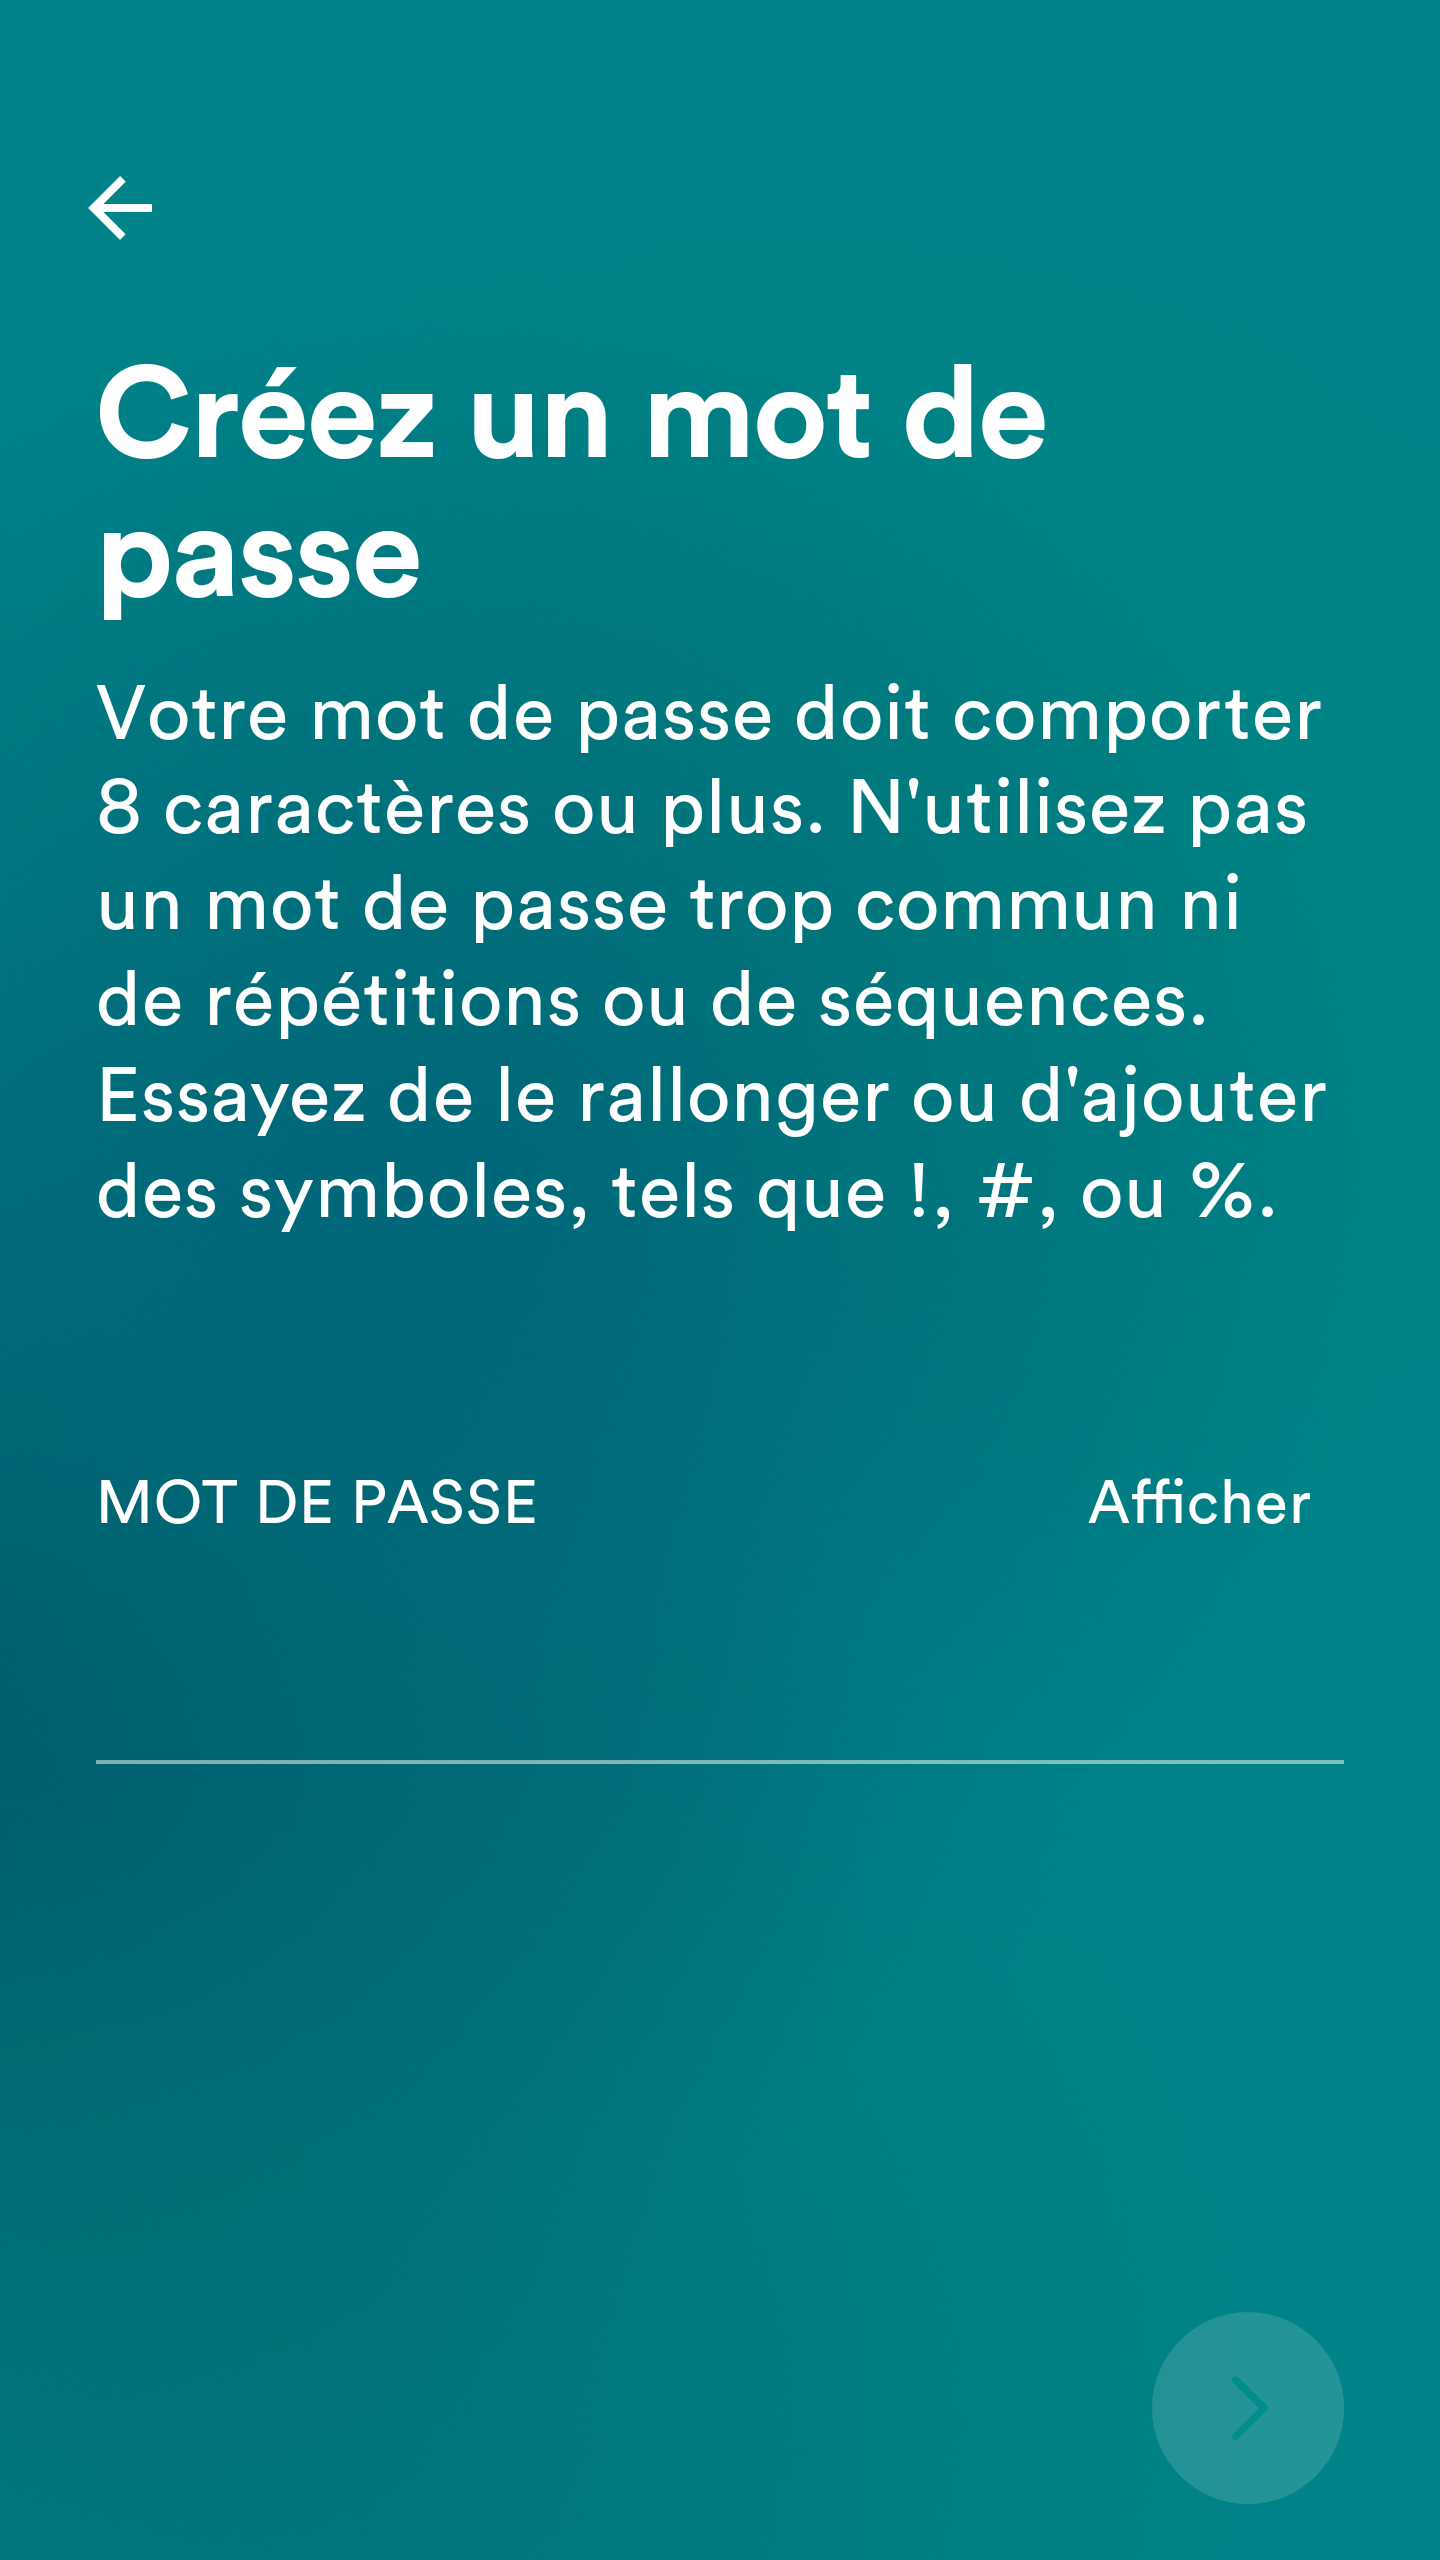
\includegraphics[width=6.5cm]{images/screen/mobile/4.png}
        \caption{Mot de passe - Inscription}
    \end{minipage}
\end{figure}

\subsection{Client Web}
\begin{figure}[H]
	\begin{center}
		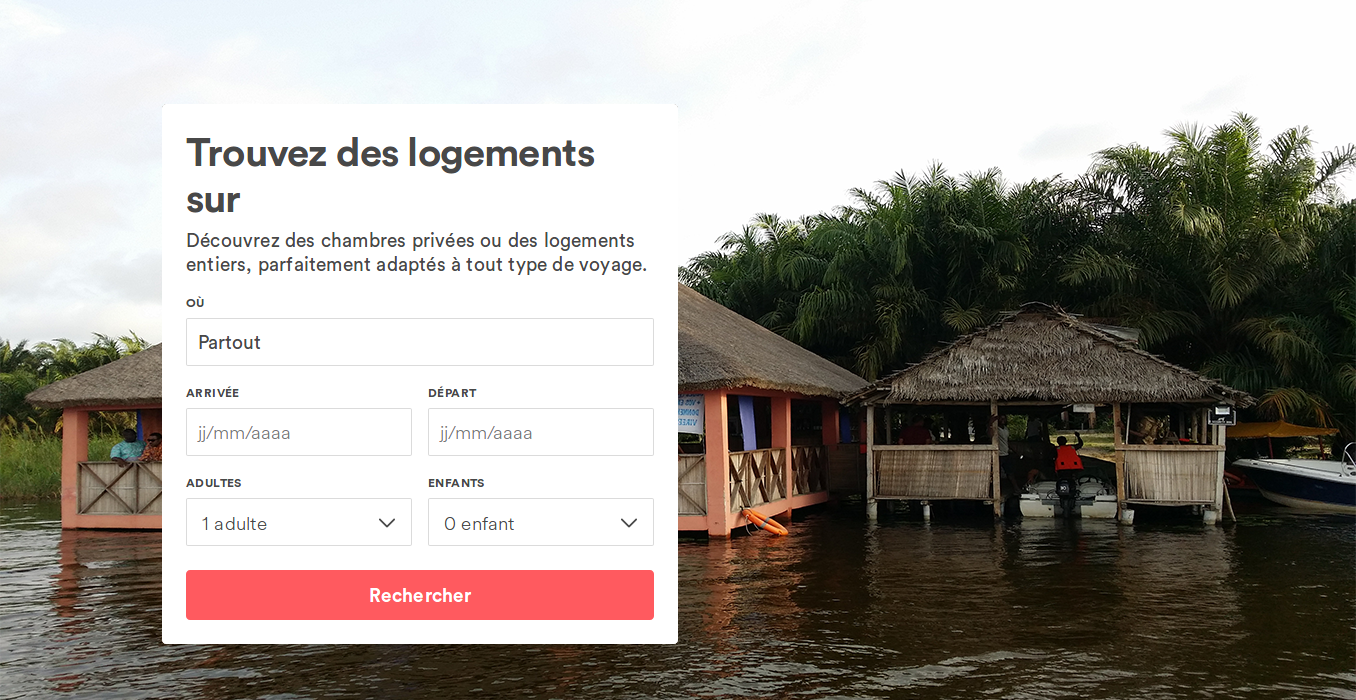
\includegraphics[width=17cm]{images/screen/web/1.png}
	\end{center}
	\caption{Accueil}
\end{figure}
\begin{figure}[H]
	\begin{center}
		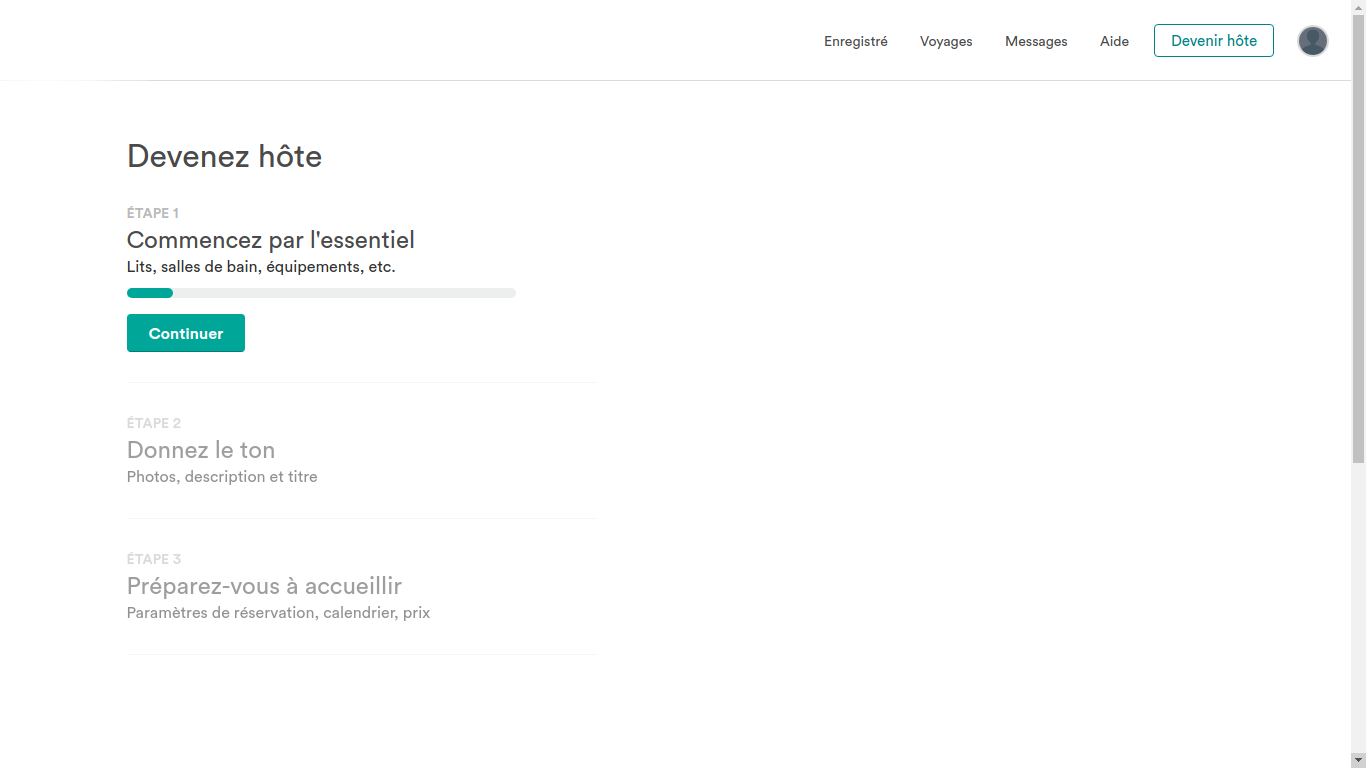
\includegraphics[width=17cm]{images/screen/web/3.png}
	\end{center}
	\caption{Devenir un hôte}
\end{figure}

\section{Déploiement de l'application}
Le déploiement de l’application et la mise en production s’est fait en continu tout au long du développement en utilisant le service Heroku\footnote{https://www.heroku.com/}.
\subsection{Heroku}
Heroku est un service de cloud computing de type PaaS\footnote{Platform-as-a-Service (plate-forme en tant que service)}. Créé en 2007, il était l'un des tout premiers services cloud. À l'origine dévolue aux applications web programmées en Ruby et utilisant Ruby on Rails, l'offre s'est ensuite étendue à d'autres runtimes : node.js, Java, Clojure, Python et Django, Scala, ainsi que PHP. Le service permet le déploiement très rapide d'applications web dans le cloud, avec une gestion très souple du scaling horizontal au travers d'un modèle de gestion des processus emprunté à Unix et adapté au Web. Côté bases de données, Heroku intègre plusieurs bases NoSQL, dont MongoDB et Redis.
L’environnement Heroku est accessible à travers la ligne de commande, via git, et un ensemble d'outils: Heroku-CLI.\\
Pour mettre en ligne les modification du projet nous avons a saisir les commandes:
\begin{lstlisting}
git add .
git commit -m 'modifications'
git push heroku master
\end{lstlisting}
Notre base de donnée est hébergée sur MongoLab un service DaaS\footnote{Database-as-a-Service}
spécialisé en hébergement MongoDB 
Ensuite nous avons essayé d'intégrer des tests (tests unitaires, tests d'intégration et tests de validation) mais cela n’a été possible faute de temps.
\\\\
Enfin nous avons acheté le nom de domaine nymeria.co ou l'application est desormais disponible.

\section{Perspectives et évolution de la plateforme}
Nous avons prévu de nombreuses améliorations pour le projet:
\begin{enumerate}
	\item Mettre en place des tests unitaires et automatiser le déploiement
	\item Achever le développement de l’API et de l'application mobile
	\item Pousser plus loin l’utilisation de React et de Redux
	\item Améliorer les algorithmes utilisés afin de faire des proposition de logement plus personnalisés et pertinentes
	\item Améliorer l’interface de l'application
	\item Intégrer les API de paiement Moov et Mtn Mobile Money
\end{enumerate}

\cleardoublepage
\phantomsection
\addcontentsline{toc}{chapter}{Conclusion}
\chapter*{Conclusion}
Le présent rapport est le résultat de notre stage effectué dans le cadre de la réalisation de notre projet de fin d’études de Licence en Architecture Logicielle au sein de l’ONG EtriLabs. Au cours de ce stage de six (6) mois, nous avons pu mettre en pratique nos connaissances théoriques acquises durant notre formation.
\\Notre projet de fin d’année avait donc pour but de mettre en place une plateforme communautaire de découverte d’expérience et de location à court terme d’appartement ou de parties d’appartement entre particuliers.
\\Nous avons, tout d’abord, entamé notre étude par l’analyse qui est une étape cruciale et nécessaire pour comprendre le problème et les plateformes déjà existantes, puis par la définition des principaux acteurs et l’identification des besoins. Elle nous a permis la conception d’une architecture de base stable. Enfin, nous avons procédé au choix justifié des technologies avant de passer à l’implémentation, qui nous a permis de développer ces applications en tenant compte de l’architecture matérielle, de l’environnement logiciel et des contraintes techniques de l’entreprise.
\\De ce qui précède, il est difficile de prétendre avoir eu une solution idéale. Toutefois, nous espérons avoir répondu tant soi peu à notre problématique. Cependant, nous sommes conscients des améliorations à faire. Nous avons prévu de travailler sur des algorithmes de compression de données afin d’améliorer les temps d’échanges sur des connexions à faibles débits. Aussi, pour la messagerie instantanée nous prévoyons d'implémenter des algorithmes d'intelligence artificielle afin de proposer de façon optimale aux visiteurs le logement parfait pour eux.
\\Nous sommes riches d’un patrimoine historique extraordinaire dont nous pouvons être fiers. Ce patrimoine doit nous permettre de développer le tourisme, un secteur capteur d’emplois et capable de faire rayonner le Bénin dans le monde. Enfin, nous avons un capital humain de grande réputation avec de nombreux Béninois qui se distinguent dans le monde entier.
%\cleardoublepage% le corps du document est termin\'e

\backmatter
\pagenumbering{Roman}

\chapter{Bibliographie et Webographie}


\begin{enumerate}
	\item Julien FONTANET, Olivier LAMBERT « Exploitez la puissance de JavaScript côté serveur ». Mars 2015 ISBN : 978-2-7460-8978-5
	\item Présidence-Bénin. « Programme d'actions du gouvernement 2016-2021 Synthèse ». Bénin Révélé, 28 | 2017.
	\item Jean-Philippe Principaud, « Le tourisme international au Bénin : une activité en pleine expansion », Les Cahiers d’Outre-Mer, 226-227 | 2004, 191-216.
	\item Ken Schwaber et Jeff Sutherland, « Scrum Guide ». \url{https://www.scrum.org/Portals/0/Documents/Scrum\%20Guides/2013/Scrum-Guide-FR.pdf} Scrum.org (consulté le 10 Novembre 2017) | 2013 p. 4.
	\item Bouhaddaoui (M. Y.) et Tarek El Allam (M.) « Etude comparative sur les méthodes de modélisation: Comparatif UML - Merise ». Ecole Nationale Supérieure d'Ingénieurs de CAEN | 2010-2011.
	\item Wikipedia, 2017a. « Merise (informatique) ». \url{https://fr.wikipedia.org/wiki/Merise\_(informatique)}, (consulté le 28 avril 2017, 12:40).
	\item Wikipedia, 2017b. « UML (informatique) ». \url{https://fr.wikipedia.org/wiki/UML\_(informatique)}, (consulté le 28 avril 2017).
	\item Le Monde Afrique « Le Bénin mise sur le tourisme et l’économie numérique ». \url{http://www.lemonde.fr/afrique/article/2016/12/21/le-benin-mise-sur-le-tourisme\:-et-l-economie-numerique\_5052437\_3212.html} LE MONDE | 21.12.2016 (consulte le 15 Decembre 2017)
	\item Dan Abramov «Tutorial: Intro To React » \url{https://reactjs.org/tutorial/tutorial.html} (consulté le 12 Juin 2017)
	\item Wikipedia « Comparison of JavaScript frameworks » \url{https://en.wikipedia.org/wiki/Comparison_of_JavaScript_frameworks} (consulté le 12 Octobre 2017)
	\item Airbnb « Airbnb Expériences » \url{https://fr.airbnb.com/experiences} (consulté le 24 Novembre 2017)
	\item Willie Yao « How We Partitioned Airbnb’s Main Database in Two Weeks » \url{https://medium.com/airbnb-engineering/how-we-partitioned-airbnb-s-main-database\:-in-two-weeks-55f7e006ff21}. Airbnb Engineers | Oct 6, 2015 (consulté le 24 Se 2017)
	\item Tobi Knaup « MySQL in the cloud at Airbnb » \url{https://medium.com/airbnb-\:engineering/mysql-in-the-cloud-at-airbnb-336e5666bc94}. Airbnb Engineers | Nov 15, 2010 (consulté le 25 Novembre 2017)
	\item Tripping « 9 Airbnb Competitors That You Should Know About » \url{https://www.tripping.com/industry/rental-companies/9-airbnb-competitors-that-you-should-know\:-about}. | Dec 08, 2016 (consulté le 24 Novembre 2017)
	\item AirbnbReview « Top 9 Airbnb Competitors and Alternatives 2017 » \url{https://medium.com/@airbnb_review/top-8-airbnb-competitors-not-who-your-might-think\:-417d6b3514e0}. Jan 16 2017 | (consulté le 30 Novembre 2017)
	\item \begin{flushleft}Valentin Pringuay « Dans les coulisses des expériences Airbnb : en route vers le futur du voyage ? » \url{http://www.numerama.com/business/212056-dans-les-coulisses\:-des-experiences-airbnb-en-route-vers-le\:-futur-du-voyage.html}. Numerama | 26 novembre 2016 (consulté le 01 Decembre 2017)\end{flushleft}
	\item Josué F. MEHOUENOU « Tourisme au Bénin: 600 milliards d’investissement et 700 000 touristes attendus d’ici 2021 » \url{https://www.lanationbenin.info/index.php/actus/159-actualites/12839-tourisme-au-benin-600-milliards-d-\:investissement-et-700-000-touristes-attendus-d-ici\:-2021}. La Nation | 10 Mar 2017 (consulté le 02 Decembre 2017)
	\item Revolunet « 2 ans avec React, Babel, Webpack et cie » \url{http://putaindecode.io/fr/articles/frontend/2016-2-ans-avec-react-babel-webpack-et-cie/}. Putain de code | Dec 1, 2016 (consulté le 24 Novembre 2017)
	\item Yves ASSOGBA, « Conception et réalisation d’une plateforme d’information, éducation et communication sur la qualité de l'eau », Ecole Nationale d’Economie Appliquée et de Management, p. 94 | Octobre 2017.
	\item Ninon KPOSSOU, « Développement d’une plateforme de gestion des rendez-vous et des dossiers médicaux dans les établissements de santé », Institut de Formation et de Recherche en Informatique, p. 44 | 2017.
	\item Shadaï ALI et Fiacre AYEDOUN, « Conception et réalisation d’une application mobile de consultation de compte souscripteurs à
	SAHAM ASSURANCE VIE BENIN », Ecole Nationale d’Economie Appliquée et de Management, p. 56 | 2017.
\end{enumerate}


\setcounter{tocdepth}{3}
\cleardoublepage
\phantomsection
\addcontentsline{toc}{chapter}{Table des matières}%ajout du sommaire dans le sommaire !
\tableofcontents
\thispagestyle{backmatter}

\end{document}